\chapter{JSIM\emph{graph}}
\label{cha:jsimgraph}
\section{Overview}
In the JMT \emph{suite} a discrete-event simulator for the
analysis of queueing network models is provided. It can be used
through two interfaces: alphanumerical (JSIM\emph{wiz}) and
graphical (JSIM\emph{graph}).

JSIM\emph{graph} is the GUI front-end to JMT simulation engine. It
helps the users to perform an evaluation study in two ways.
Firstly, critical statistical decisions, such as transient
detection and removal, variance estimation, and simulation length
control, have been \emph{completely automated}, thus freeing the
users from taking decisions about parameters s/he may not be
familiar with. The simulation is automatically stopped when all
performance indexes can be estimated with the required accuracy.
Secondly, a user-friendly graphical interface allows the user to
describe, both the network layout and the input parameters.
Furthermore, the graphical interface also provides support for the
use of advanced features (several of them are for networks with
very general characteristics, usually referred to as
\emph{non-product-form} networks) like fork and join of customers,
blocking mechanisms, regions with capacity constraints on
population, state-dependent routing strategies, user-defined
general distributions, import and reuse of log data. A module for
\emph{What-If Analysis}, where a sequence of simulations is run
for different values of control parameters, particularly useful in
capacity planning, tuning and optimization studies, is also
provided.

The simulation engine performs on-line the statistical analysis of
measured performance indices, plots the collected values, discards
the initial
transient periods and computes the confidence intervals.\\
Network topologies implemented and solved using JSIM\emph{graph}
can be exported in vector (e.g., eps, pdf) or raster (e.g., jpeg,
png) image formats.\\

\ \\
\noindent \textbf{\large Main Features}\\
\noindent \textbf{Arrival rates} for open classes of customers
generated by Source stations and station \emph{service times} (for
any type of station in open and closed models) can be generated
according to the following distributions: Burst (General),
Constant, Erlang, Exponential, Gamma, Hyperexponential, Normal,
Pareto, Poisson,
Student-T, Uniform \\

\noindent \textbf{Queueing discipline}: the following strategies
are available:  First Come First Served, FCFS with priority, Last
Come First Served, LCFS with priority\\

\noindent \textbf{Routing} of the customers in the network, i.e.,
the path followed by the requests among the resources, can be
described either probabilistically or according to the following
strategies: Fastest service, Least utilization, Random, Round
robin, Join the Shortest Queue, Shortest response time (the values
of the control parameters are evaluated on the stations connected
in output to the considered one). These strategies can be further
combined among themselves through the use of a \emph{routing
station}.\\

\noindent \textbf{Other peculiar features} of the simulator are:
\vspace{-0.2cm}
\begin{itemize*}
    \item Load dependent service time strategies
    \item Fork-and-join stations to model parallelism
    \item Simulation of complex traffic pattern and service times (e.g., burst)
    \item Blocking regions (in which the number of customer is limited)
    \item What-if analysis (with various control parameters)
    \item Customization of default values
    \item Import/Export of the model from/to JMVA, the exact solver (when
    the required analytic assumptions are satisfied)
    \item Logging of the data flowing in any part of the model
    (\emph{Logger} station)
    \item Graphical visualization of the evaluated performance
    indices together with their confidence intervals
    \item automatic transient detection and removal
    \item automatic stop of the simulation when all performance
    metrics can be estimated with the required accuracy.
\end{itemize*}
JSIM\emph{graph} has a modular Java-based architecture that allows
the introduction of new Java classes in the simulation engine
without any modification to the source codes of the other classes.

\section{The home window} In the initial window of the
JSIM\emph{graph} (\autoref{fig:jsimg:Classes}), all the icons in
the toolbar except the first two (\texttt{Create a new model} and
\texttt{Open} a previously saved model) are inactive. Choosing
\texttt{Create a new model} from the toolbar or \texttt{New} from
the \texttt{File} menu bar activates the other icons in the
toolbar.
\begin{figure}[htbp]
    \begin{center}
        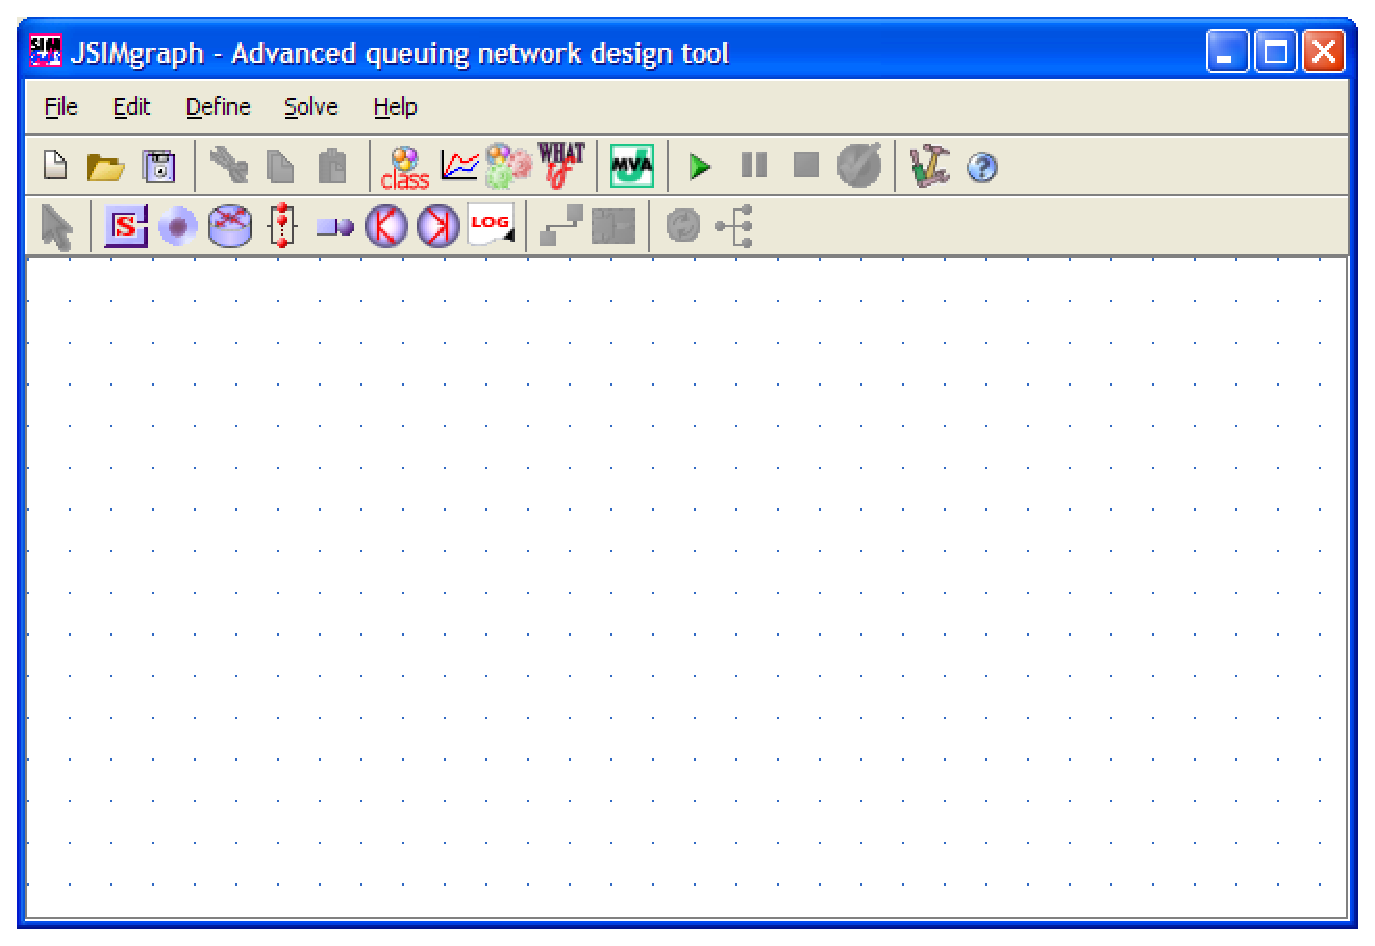
\includegraphics[scale=.5]{img/jsimg/2.1.eps}
    \end{center}
    \caption{The home window of JSIM\emph{graph}}
    \label{fig:jsimg:Classes}
\end{figure}
From \autoref{fig:jsimg:Classes}, we can see that the home window
has a \emph{menu bar} and \emph{two toolbars}. The menu bar has 5
menus: \texttt{File, Edit, Define,
Solve, Help}.\\

\noindent{\textbf{The \emph{first} toolbar has the following
icons:}}\\

\includegraphics[scale=.5]{img/jsimg/new.eps} Create a new model\\

\includegraphics[scale=.5]{img/jsimg/open.eps} Open a previously saved
model\\

\includegraphics[scale=.5]{img/jsimg/save.eps} Save the current
model\\

\includegraphics[scale=.5]{img/jsimg/cut.eps} Cut\\

\includegraphics[scale=.5]{img/jsimg/copy}
Copy\\

\includegraphics[scale=.5]{img/jsimg/paste.eps} Paste\\

\includegraphics[scale=.5]{img/jsimg/definecustclasses.eps} Define customer
classes\\

\includegraphics[scale=.5]{img/jsimg/defineperformanceindices.eps} Define the performance
indices to be evaluated and plotted\\

\includegraphics[scale=.5]{img/jsimg/defineSimulationParameters.eps} Define simulation
parameters\\

\includegraphics[scale=.5]{img/jsimg/whatIf} Define What-if analysis
parameters\\

\includegraphics[scale=.5]{img/jsimg/exportToJMVA} Export the current model to
JMVA\\

\includegraphics[scale=.5]{img/jsimg/play} Start simulation
model\\

\includegraphics[scale=.5]{img/jsimg/pause} Pause simulation\\

\includegraphics[scale=.5]{img/jsimg/stop}
Stop simulation\\

\includegraphics[scale=.5]{img/jsimg/showResultsWindow} Show simulation results
window\\

\includegraphics[scale=.5]{img/jsimg/defineDefaults} Define new default values of model
parameters\\

\noindent{\textbf{The \emph{second} toolbar has the following icons:}}\\

\includegraphics[scale=.5]{img/jsimg/select}Select\\

\includegraphics[scale=.5]{img/jsimg/insertSource} Insert a source
station\\

\includegraphics[scale=.5]{img/jsimg/insertSink} Insert a sink station\\

\includegraphics[scale=.5]{img/jsimg/insertRouter} Insert a routing
station\\

\includegraphics[scale=.5]{img/jsimg/insertDelay} Insert a delay station\\

\includegraphics[scale=.5]{img/jsimg/insertServer} Insert a queueing station\\

\includegraphics[scale=.5]{img/jsimg/insertFork} Insert a fork node\\

\includegraphics[scale=.5]{img/jsimg/insertJoin}  Insert a join node\\

\includegraphics[scale=.5]{img/jsimg/logger}  Insert a logger station\\

\includegraphics[scale=.5]{img/jsimg/connect}  Connect two elements\\

\includegraphics[scale=.5]{img/jsimg/addStationToNFCR}  Add selected
stations to a new Finite Capacity
Region\\

\includegraphics[scale=.5]{img/jsimg/rotate}  Rotate the component\\
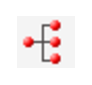
\includegraphics[scale=.5]{img/jsimg/optimizeGraph}  Optimize the graph\\

\section{Working with the graphical interface}
\subsection{Defining a new model} \label{sec:DefiningANewModel}
To define a new model the following steps have to be performed.\\
1. Draw the network (click and drop) \\
2. Define \emph{Customer Classes} and select the \emph{Reference Station} for each
class\\
3. Set the parameters for each object\\
4. Select the performance indices to be collected and evaluated\\
5. If needed, insert one or more \emph{Finite Capacity Regions} (FCR)\\
6. Choose or change the simulation parameters\\
7. Enable \emph{What-If Analysis} and set its parameters, if required\\
8. Start the simulation\\
9. If diagnostic errors are detected, click on them and the
related window that allows immediately to fix them will be
shown.\\

\noindent{\textbf{Step 1: Create the new model}}

To draw a new network, select

\includegraphics[scale=.5]{img/jsimg/new.eps} or choose
\texttt{New} from \texttt{File menu}.  A white area in which the
model should be drawn will be shown. Utilize the pre-defined objects
like queueing station, delay,
source, sink, logger, connection, routing station and fork/join.

\noindent{\textbf{Step 2: Define customer classes}}

In all the networks implemented, one or more \emph{Customer Classes} must
be defined. To describe them, see \autoref{sec:DefineClasses} -
"\emph{Defining Customers Classes}" and parameterize the classes to use.\\
For each class of customers, a \emph{Reference Station} should be
set. This station is used to compute the system throughput for
each class (i.e., the number of customers of that class that flow
through the system in a time unit). It is a \emph{required
parameter} in order to compute correctly the simulation results.
If a simulation is started without its prior definition, an error
message will appear.

\noindent{\textbf{Step 3: Define station parameters}}

All the stations have default parameters. The proper parameters of
the objects should be defined: either the numeric values or the
qualitative parameters such as routing strategy, queueing policy,
maximum number of customers in a FCR region, etc. See
\autoref{defnettop} - "\emph{Defining Network Topology}" for
details.

\noindent{\textbf{Step 4: Define performance indices}}

The performance indices that will be evaluated during the
simulation should be selected. Select the indices and set the
class and the station which each index refers to. See
\autoref{perfinde} - "\emph{Performance Indices}" for details.

\noindent{\textbf{Step 5: Define a Finite Capacity Region}}

A \emph{F}inite \emph{C}apacity \emph{R}egion (FCR) is a section
of the model, that may consists of one or more stations, in which
the number of customers is limited. Several FCRs can be defined in
a network, provided that they \emph{do not} overlap. See
\autoref{defcap} "\emph{Finite Capacity Region (FCR)}" to
learn how to set this type of region.

\noindent{\textbf{Step 6: Setting simulation parameters}}

The parameters that control the simulation and the initial state
of the network should be defined. See \autoref{modifpa}
"\emph{Modification of the parameters}" for details.

\noindent{\textbf{Step 7: Enabling a What-If Analysis}}\\
If you decide to set up a What-If Analysis read
\autoref{whaif}.

\noindent{\textbf{Step 8: Start the simulation}}\\
Press

\includegraphics[scale=.5]{img/jsimg/play} or select
\texttt{Simulate} from the \texttt{Solve} menu to start the
simulation.  Before starting the simulation, a check if the
defined network is correct is performed, and the errors detected
(fatal or warning) are shown.  The results of a simulation are
described in \autoref{ressults}.

\noindent{\textbf{Step 9: Fatal Errors and Warning Messages}}\\
The detected errors and warning messages are shown in
\autoref{erwar}.\\



\subsection{Defining the classes of customers} \label{sec:DefineClasses}
 The workload intensity is described by one of the following
 parameters:\\
$\lambda$ the arrival rate (for open models)\\
N the population size (for closed models).\\
In \emph{open} models the workload intensity is specified by the
parameter $\lambda$, i.e., the rate at which requests (customers)
arrive at the system. In these type of models there is an infinite
stream of arriving customers and the customer population, i.e.,
the number of customers in execution, varies over time. Customers
that have completed their execution leave the system (and reach a
\emph{sink station}). The class of customers of an open model is
also referred to as \emph{Open Class}.\\
 In \emph{closed} models the workload intensity is specified by a
parameter N, indicating the average number of jobs (customers) in
execution. In these models the population is fixed, i.e., N is
kept constant. Customers that have completed their service are
considered as if they left the model and have been replaced
immediately by a new customer. The class of customers in execution
in a closed model is also referred as \emph{Closed Class}.
 Multiple class models consist of N customer classes, each of which
 has its own workload intensity and its own service demand at each center.
 Within each class, the customers are indistinguishable, i.e., statistically
 equal. Models, in which the customers belong to both of the two types of
 classes, open and closed, are referred to as Mixed models.
The parameters defining the two types of classes are given below.
\begin{itemize*}
\item \textbf{Open Classes parameters:} priority, interarrival
time distribution, reference station, service time distributions
of the stations \item \textbf{Closed Classes parameters:}
priority, population value, reference station, service time
distributions of the stations. \end{itemize*}

 The classes
of customers identify different customer behavior and
characteristics, such as the type (closed or open), the size of
the customer population (for closed classes) or the interarrival
time distribution (for open classes), the path among the
resources, the service time required.

They can be set from the \texttt{Define} menu by choosing
\texttt{Customer Classes}. The following panel will be shown.

\begin{figure}[htb]
    \begin{center}
        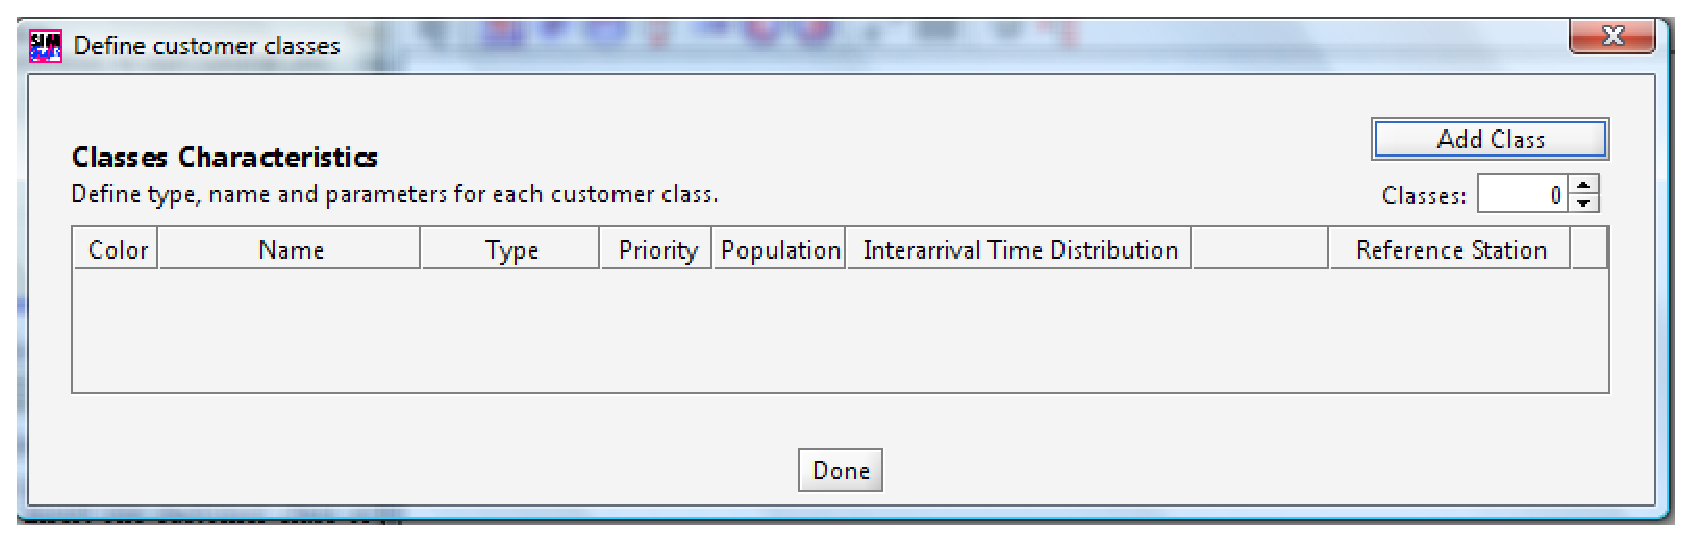
\includegraphics[scale=.5]{img/jsimg/3.1.eps}
    \end{center}
    \caption{Window for the definition of the classes of customers}
    \label{fig:jsimg:defclwin}
\end{figure}

Classes must be explicitly added to the model, either one at a
time by clicking the \texttt{Add Class} button, or by selecting
directly the desired final number of classes from the
\texttt{Classes} counter. The newly added classes will be listed
with default parameters.

Double click on the default name (i.e., Class0, Class1, etc.) to
change it. Each new class has a priority in the system. A smaller
number indicates a lower priority. Default value is 0, it can be
changed by double clicking on the corresponding area. In this
panel you can insert either one or multiple
customer classes.\\

\textbf{Defining Open Classes}\\
After adding a class and set its name and priority, you must
select the type of the class. Classes are created \emph{Closed by
default}, so if you want an \emph{Open} class, select the type
\emph{Open} from the \texttt{Type} menu.
\begin{figure}[htb]
    \begin{center}
        
\includegraphics[scale=.5]{img/jsimg/3.2.eps}
    \end{center}
    \caption{Selection of the type of the class}
    \label{fig:typeclass}
\end{figure}

Now the class characteristics should look like \autoref{fig:classchar}.

\begin{figure}[htb]
    \begin{center}
        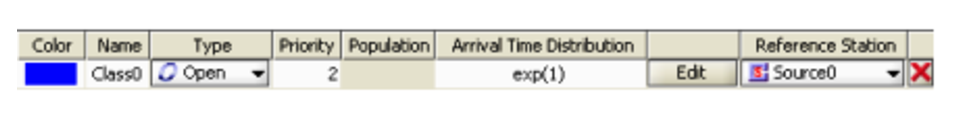
\includegraphics[scale=.5]{img/jsimg/3.3.eps}
    \end{center}
    \caption{Class characteristics window}
    \label{fig:classchar}
\end{figure}

Open classes describe customer populations that vary over time.
They are characterized by the probability distribution of the
interarrival time of customers arriving at the system. The
\emph{default} Interarrival Time Distribution is \emph{exp(1)}
(Exponential Distribution with $\lambda$ =1). To change the
Interarrival Time Distribution, click the \texttt{Edit} button.
\begin{figure}[htb]
    \begin{center}
        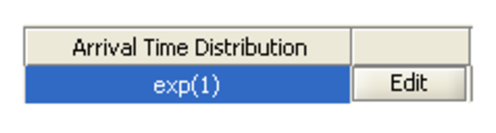
\includegraphics[scale=.5]{img/jsimg/3.4.eps}
    \end{center}
    \caption{Definition of the interarrival time distribution and its parameters (\texttt{Edit} button)}
    \label{fig:defclasschar}
\end{figure}

The following window will appear:
\begin{figure}[htb!]
    \begin{center}
        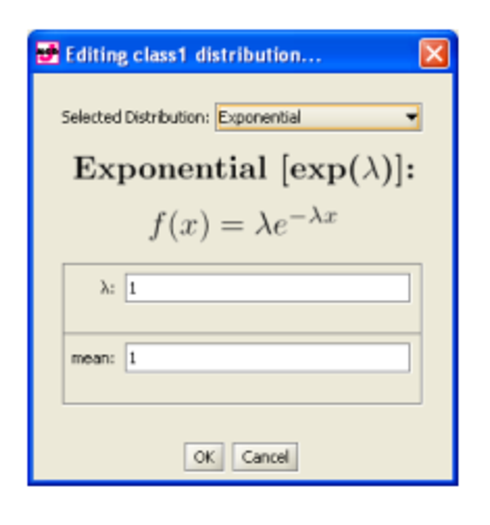
\includegraphics[scale=.5]{img/jsimg/3.5.eps}
    \end{center}
    \caption{Window for the editing of the distribution of interarrival times}
    \label{fig:editdistrib}
\end{figure}

\noindent{Click on the \texttt{Selected Distribution} drop down
menu to
choose one of the following distributions:}\\
\emph{Burst (General)\\
Burst (MMPP2)\\
Constant\\
Erlang\\
Exponential\\
Gamma\\
Hyperexponential\\
Normal\\
Pareto\\
Poisson\\
Replayer\\
StudentT\\
Uniform.\\
} For each distribution the correct values of the
parameters should be described, \emph{default} values can eventually be
used. Parameters that are related each others are automatically
updated when one of them is modified. For example, for an
\emph{Erlang} distribution, when you set the ($\alpha, r$) pair, the
($mean, c$) pair is automatically set to the correct values. The
\emph{Replayer} distribution
allows the user to use trace of data collected from real experiments.\\
Click \texttt{OK} to return to \texttt{Class parameters} definition.\\
The final step of a class definition is the identification of the
\emph{Reference Station}, i.e., the station of the model used to
compute the system throughput and response time of a class. It can be
selected from
the \texttt{Reference
Station} menu (\autoref{fig:selrefstat}). For
\emph{Open Classes}, \emph{only} one of the stations of
\texttt{Source} type can be selected as \emph{Reference Station}.
\begin{figure}[htb!]
    \begin{center}
        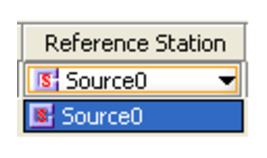
\includegraphics[scale=.5]{img/jsimg/3.6.eps}
    \end{center}
    \caption{Selection of the Reference Station for an open class of customers}
    \label{fig:selrefstat}
\end{figure}\\

\textbf{Defining Closed Classes}
\begin{figure}[htb]
    \begin{center}
        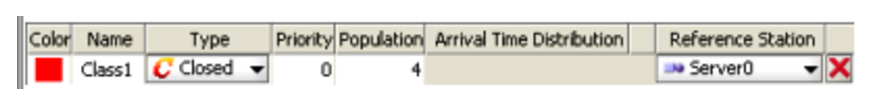
\includegraphics[scale=.5]{img/jsimg/3.7.eps}
    \end{center}
    \caption{Closed class definition parameters}
    \label{fig:closecldef}
\end{figure}


By \emph{default} Classes are created as \emph{Closed}. Priority
can be changed as in the case of Open class (the default value is
0, the minimum). The population size (also referred to as $N$) is
the parameter that characterizes a closed class.  For a closed
class N is constant and does not change during the execution of
the simulation. Its \emph{default} value is 1 and it may be
changed by clicking on the corresponding area in the class
properties matrix.
\begin{figure}[htb]
    \begin{center}
        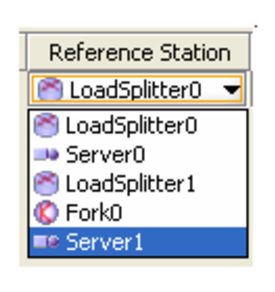
\includegraphics[scale=.5]{img/jsimg/3.8.eps}
    \end{center}
    \caption{Selection of a Reference Station for a closed class of customers}
    \label{fig:closerefstat}
\end{figure}
A Reference Station for the class \emph{must} be selected from the
\texttt{Reference Station} menu. With a closed class all the type
of stations can be selected but neither a \emph{Source} nor a
\emph{Sink}. The \emph{Reference Station} is used to compute the
system throughput and response time for the class considered.

\section{Distributions}
\label{distns}
Open class models are workloads where the number of
requests in the system fluctuates over time and new  requests
arrive at the system as if generated by an infinite source. The
arrival pattern can be described by a probability distribution
simple or very complex. It is often used the distribution of the
\emph{inter-arrival} times of consecutive requests, or customers.

A probability distribution $f(x)$ can be characterized by:\\
\emph{Mean} (if it exists):
\[
E[X]\; =\;\int_{-\infty}^{\infty} x\, f(x)\,dx
\]
\emph{Variance} (if it exists):
\[
Var[X] = \; \int_{-\infty}^{\infty} (x-E[X])^2 f(x)\; dx \;\; =
E[X^2] - E[X]^2
\]
\emph{Coefficient of variation c} (when mean and variance exist
and mean is not 0):
\[
c\; = \; \frac{\sqrt{variance}}{mean}
\]
The following probability distributions are currently supported.\\

\textbf{\emph{Burst (General)} distribution}\\
The Burst (General) distribution is a complex distribution
obtained combining two different distributions. It allows the
simulation of complex patterns of arrivals and may be suitable for
simulating the load generated by web 2.0 applications. A Burst
(General) distribution consists of two different types of
intervals (A and B) independent among each other. For both the
interval types the following parameters have to be specified:
\begin{itemize*}
\item the \emph{probability} of \emph{occurrence} of that type of
interval in the generated stream \item the \emph{length
distribution} for that type of intervals \item the distribution of
the \emph{values} generated into each interval.
\end{itemize*}
The Burst (General) distribution behaves as follows. As soon as
the simulation starts, an interval is chosen based on the
specified probability of occurrence. If, for example, interval
type A has probability of occurrence of 0.7 and interval B has
0.3, then an interval of type A is chosen with 70\% probability.
In order to determine the duration of an interval, an event from
the interval-length distribution is obtained. The distribution of
the events of an interval is then used to compute the arrival time
of customers or the service time of a station, depending on where
the Burst (General) distribution is used. As soon as the interval
ends, a new interval is chosen based on the given probability as
before.

\autoref{fig:strburdistr} shows the concept idea of the Burst
(General) distribution, clarifying the role of the occurrence
probability and the role of the interval length.
\begin{figure}[htb]
    \begin{center}
        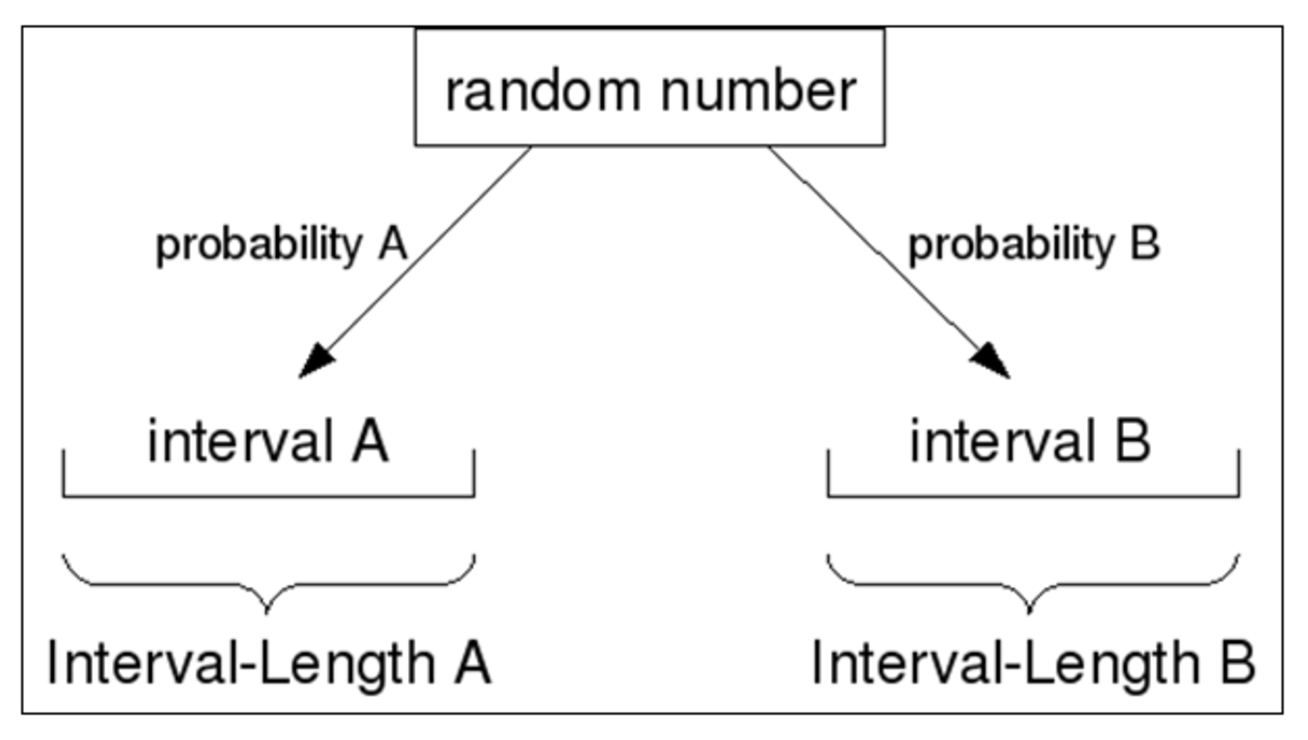
\includegraphics[scale=.5]{img/jsimg/4.1.eps}
    \end{center}
    \caption{Main structure of the \emph{Burst (General)} distribution consisting
    of two type of intervals with independent statistical characteristics}
    \label{fig:strburdistr}
\end{figure}\\

\textbf{\emph{Burst (MMPP2)} (mmpp2($\sigma_0,\sigma_1,\lambda_0,\lambda_1$)) distribution}\\
A MMPP(2) is a continuous-time Markov chain that jumps between two
states and the active state determines the current rate of service. For example, one state may be
associated with slow inter-arrival times (state 0), the other may have fast
inter-arrival times (state 1). As time passes, the MMPP(2) jumps several times between the slow state 0 and
the fast state 1.

In JMT, the MMPP(2) is parameterized by four rates: $\sigma_0$,  $\sigma_1$,
$\lambda_0$, and $\lambda_1$ (see \autoref{fig:mmpp2}). While in state $0$, the MMPP(2) generates
arrivals with rate $\lambda_0$ or jumps to state $1$ with rate $\sigma_0$; in state 1 the arrival
and jump rates are $\lambda_1$ and $\sigma_1$, respectively. This can be equivalently stated as follows: in state $0$ a random number with exponential distribution having rate $\lambda_0+\sigma_0$ is drawn, then with probability $\lambda_0/(\lambda_0+\sigma_0)$ is the arrival of a new job (or equivalently the completion of its service if the MMPP(2) is used as a service process), while with probability $\sigma_0/(\lambda_0+\sigma_0)$ \emph{without} any job arrival or service completion; the case of state $1$ is similar.

A MMPP(2) can be parameterized to have a predefined mean, $c^2$, skewness, decay rate of the autocorrelation. Given these four parameters, there are closed-form formulas to obtain the corresponding values
of  $\sigma_0$,  $\sigma_1$, $\lambda_0$, and $\lambda_1$. For example the mean is
related to the rates of the MMPP(2) by

\[mean=\frac{\sigma_0+\sigma_1}{\lambda_0\sigma_1+\sigma_0\lambda_1}\]

while the decay rate of the autocorrelation that controls the burstiness is
\[
decay~rate=\frac{\lambda_0\lambda_1}{\lambda_0\lambda_1+\lambda_0\sigma_1+\sigma_0\lambda_1}.
\]

In particular, a large decay rate ($>0.9$) creates large bursts of arrivals/service completions.
The reader could find additional details on how to fit a MMPP(2) for example in \cite{CasZS07} and references therein.

\textbf{example 1)}$\lambda_0=\lambda_1=5$ is an exponential distribution for all
choices of $\sigma_0$ and $\sigma_1$

\textbf{example 2)}$\lambda_0=1.4346$, $\lambda_1=0$, $\sigma_0=0.0139$, $\sigma_1=0.0319$
is an hyperexponential with mean$=1$, $c^2=20$, $p=0.99$. since the
hyperexponential has no burstiness, here the autocorrelation
coefficients are equal to zero.

\textbf{example 3)} $\lambda_0=12$, $\lambda_1=0.0879$, $\sigma_0=0.0010$,
$\sigma_1=0.0001$ is a MMPP(2) with burstiness. The mean is 1, $c^2$=20,
skewness$=7.31$, lag-1 autocorrelation coefficient is $0.4745$. Since for
a MMPP(2) the autocorrelation is always less than $0.5$, this is an
example of a process with very large burstiness.

\begin{figure}[htb]
    \begin{center}
        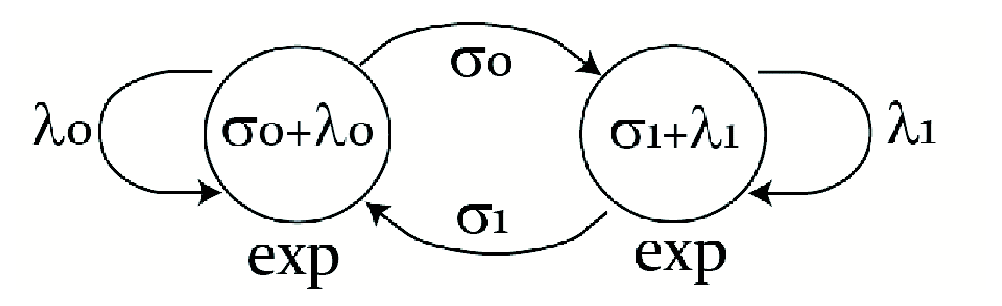
\includegraphics[scale=.5]{img/jsimg/mmpp2.eps}
    \end{center}
    \caption{Main structure of the \emph{Burst (MMPP2)} distribution}
    \label{fig:mmpp2}
\end{figure}

\textbf{\emph{Constant} (Const(k)) distribution}\\
 This distribution
describes a constant (deterministic) flow of customers, arriving
exactly every \emph{k} time units. The probability density function is:
\[ f(x) = \left\{ \begin{array} {ll}
          1   &   \mbox{ $x=k$ } \\
          0   &   \mbox{$x\neq{k}$}
                 \end {array}
\right.   \] The only parameter that should be specified is the
\emph{mean}, equal to \emph{k}.
\begin{figure}[htb]
    \begin{center}
        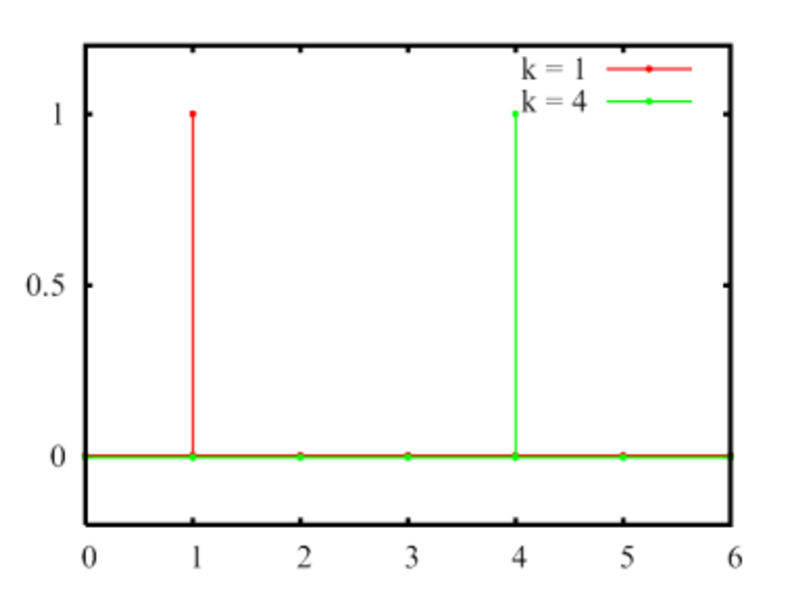
\includegraphics[scale=.5]{img/jsimg/4.2.eps}
    \end{center}
    \caption{\emph{Constant} distributions for two different mean values}
    \label{fig:constk}
\end{figure}\\

\textbf{\emph{Erlang} (erl($\alpha$,r)) distribution}\\
The \emph{Erlang} distribution is a continuous distribution, with
two parameters: the \emph{shape} \emph{r}, an integer value, and the
\emph{rate}
$\alpha$, a real value. It is a special case of a Gamma
distribution with integer shape parameter. The probability density
function is:
\[
f(x)\; = \; \frac{\alpha^r}{\Gamma(r)} \; x^{r-1} \; e^{-\alpha x}
\]
$\Gamma(r)$ is called Eulero function and when \emph{r} is a non
null positive integer, as in the case of the Erlang distribution,
the Eulero function reduces to $\Gamma(r)= (r-1)!$.\\
A random variable with Erlang distribution of order \emph{r} can
be obtained as a sum of \emph{r} exponentially distributed random
variables with mean $1/r \alpha$ (see \autoref{fig:simErl}).
\begin{figure}[htb]
    \begin{center}
        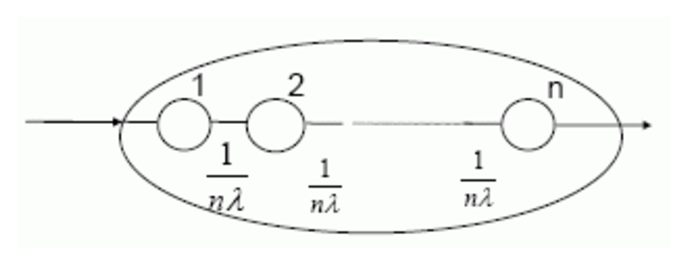
\includegraphics[scale=.5]{img/jsimg/4.3.eps}
    \end{center}
    \caption{Simulation of an Erlang distribution with a sequence of exponential stages}
    \label{fig:simErl}
\end{figure}
When the values of $\alpha$ and \emph{r} are changed, the system
will automatically recompute the mean = r/$\alpha$ and the
variance $Var = r/\alpha^2$. A family of probability density
functions that illustrate the impact of various ($\alpha$, r)
pairs is shown in \autoref{fig:famErl}.
\begin{figure}[htb]
    \begin{center}
        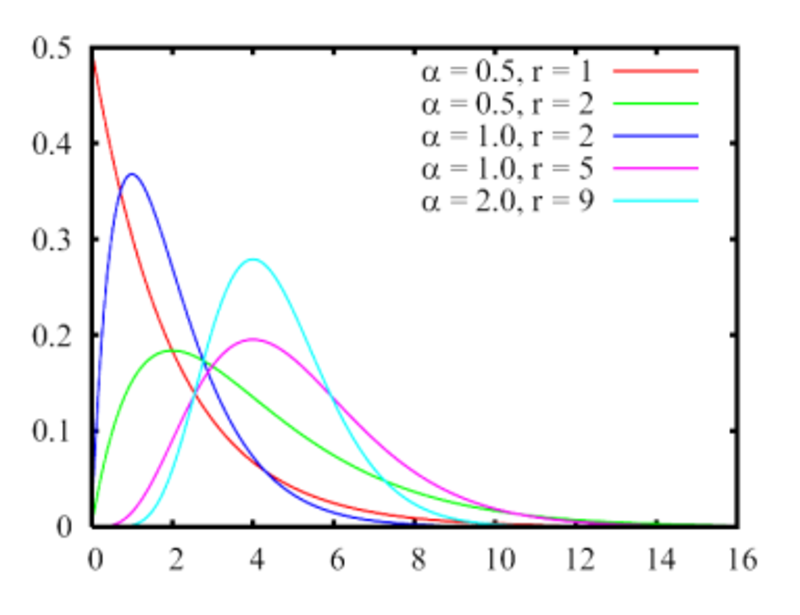
\includegraphics[scale=.5]{img/jsimg/4.4.eps}
    \end{center}
    \caption{A family of Erlang distributions with different values of the
    parameters ($\alpha$, \emph{r})}
    \label{fig:famErl}
\end{figure}\\


\textbf{\emph{Exponential} (exp($\lambda$)) distribution}\\
 This
is a continuous probability distribution where $\lambda >$ 0 is
the distribution parameter, often called the \emph{rate}
parameter; the distribution is defined in the interval
[0,$\infty$). The probability density function is:
\[ f(x) = \left\{ \begin{array} {ll}
          \lambda e^{- \lambda x}   &   \mbox{ $x \geq 0$ } \\
          0   &   \mbox{$x < 0$}
                 \end {array}
\right.   \]

The exponential distribution is used to model Poisson processes.
The time interval between two consecutive events generated by a
Poisson process can be described by an exponential random variable
with parameter $\lambda$.\\
The parameter $\lambda$ is a real number, the mean value is
 given by $1/\lambda$, the variance is given by $1/\lambda^2$.

A family of exponential density functions with different values of
$\lambda$ is shown in \autoref{fig:famExp}.
\begin{figure}[htb]
    \begin{center}
        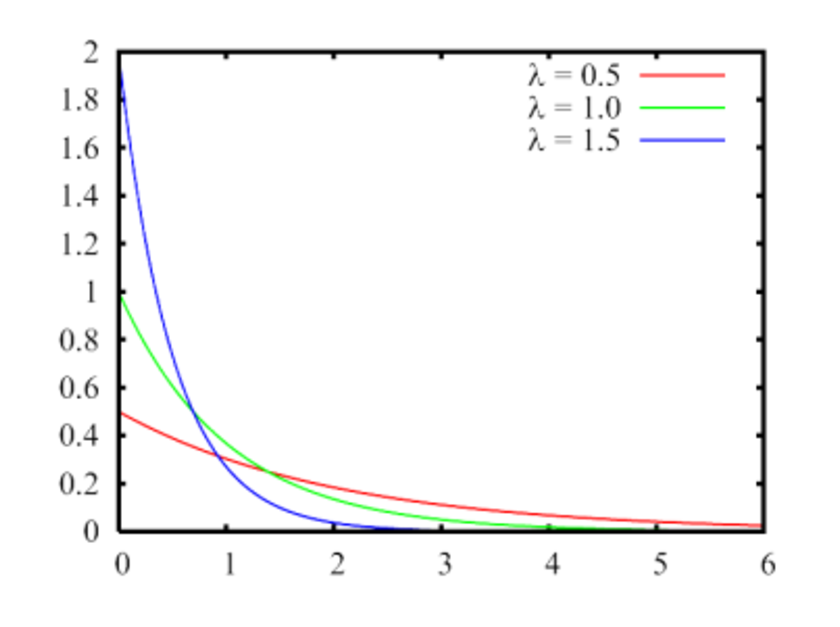
\includegraphics[scale=.5]{img/jsimg/4.5.eps}
    \end{center}
    \caption{Exponential density functions with different mean (1/$\lambda$) values)}
    \label{fig:famExp}
\end{figure}\\

\textbf{\emph{Gamma} (gam($\alpha,\lambda$)) distribution}\\
The \emph{Gamma} is a continuous probability distribution with two
parameters: the shape $\alpha$ and the scale $\lambda$, both real
numbers. The probability density function is:
\[
f(x)\; = \; \frac{x^{\alpha-1}}{\Gamma(\alpha) \lambda^\alpha} \;
\; e^{- x/\lambda}
\]
where $\Gamma(t)$ is the Eulero function. When the Gamma
distribution is selected, the user can either provide $\alpha$ and
$\lambda$ or the distribution mean equal to $\alpha \lambda$ and
the variance $\alpha \lambda^2$. A family of probability density
functions is shown in \autoref{fig:famGam}, for a set of $\alpha$
and $\lambda$ values.
\begin{figure}[htb]
    \begin{center}
        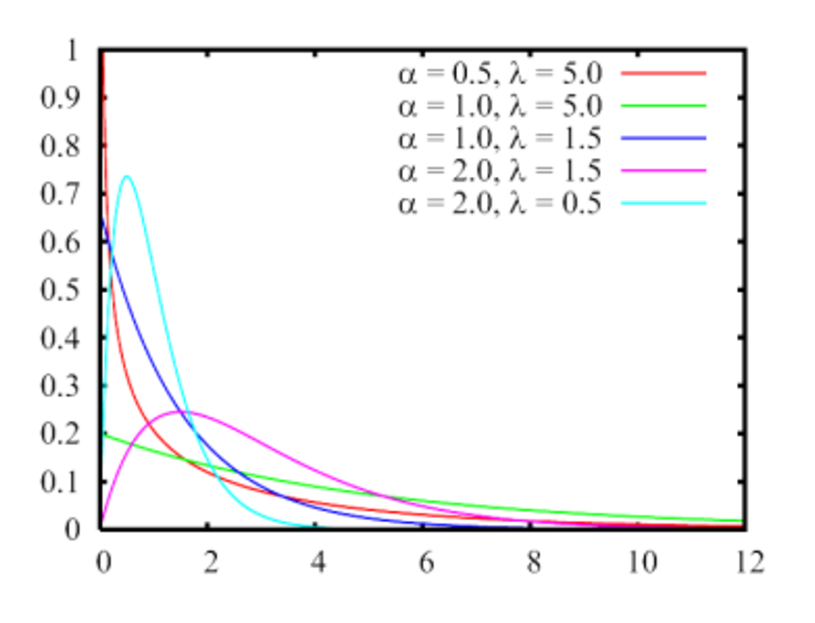
\includegraphics[scale=.5]{img/jsimg/4.6.eps}
    \end{center}
    \caption{\emph{Gamma} density functions for different values of $\alpha$ and $\lambda$}
    \label{fig:famGam}
\end{figure}\\

\textbf{\emph{Hyperexponential} (hyp(p,$\lambda_1,\lambda_2$))
distribution}\\
A hyperexponential distribution describes a random variable
characterized by a variability higher with respect to an
exponential one with the same mean. It is the result of a weighted
sum of two independent exponentially distributed random variables,
with parameters $\lambda_1$ and $\lambda_2$ respectively. The
weight \emph{p} is the probability  that the random variable
behaves like the exponential variable with parameter $\lambda_1$
and \emph{1-p} that it behaves like the exponential variable with
parameter $\lambda_2$. The probability density function is:
\[ f(x) = p \; \lambda_1 e^{- \lambda_1 x}\; + \;
(1-p) \; \lambda_2 e^{- \lambda_2 x}
\]
\begin{figure}[htb]
    \begin{center}
        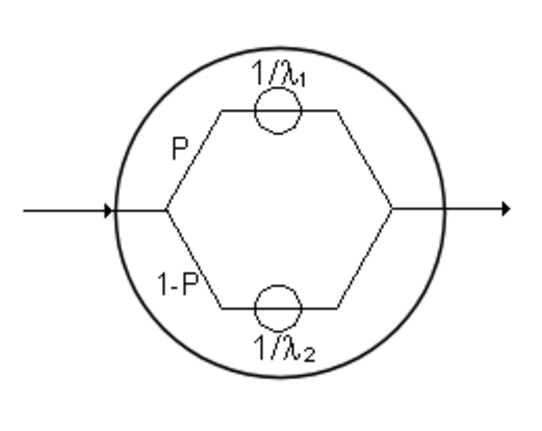
\includegraphics[scale=.5]{img/jsimg/4.7.eps}
    \end{center}
    \caption{Generation of the values of an hyperexponential function
    through two exponential stages in parallel}
    \label{fig:genHyper}
\end{figure}
When this distribution is used to model customer interarrival time
or a station service time, with probability \emph{p} the next
interval before a new arrival (or the next service time) is
distributed like the upper server in \autoref{fig:genHyper} the
figure above while with probability \emph{1-p} it will be
distributed like the lower server.

A family of hyperexponential density functions is shown in
\autoref{fig:famHyper}. Note that when $\lambda_1 = \lambda_2$,
the hyperexponential reduces to a simple exponential.\\

\begin{figure}[htb]
    \begin{center}
        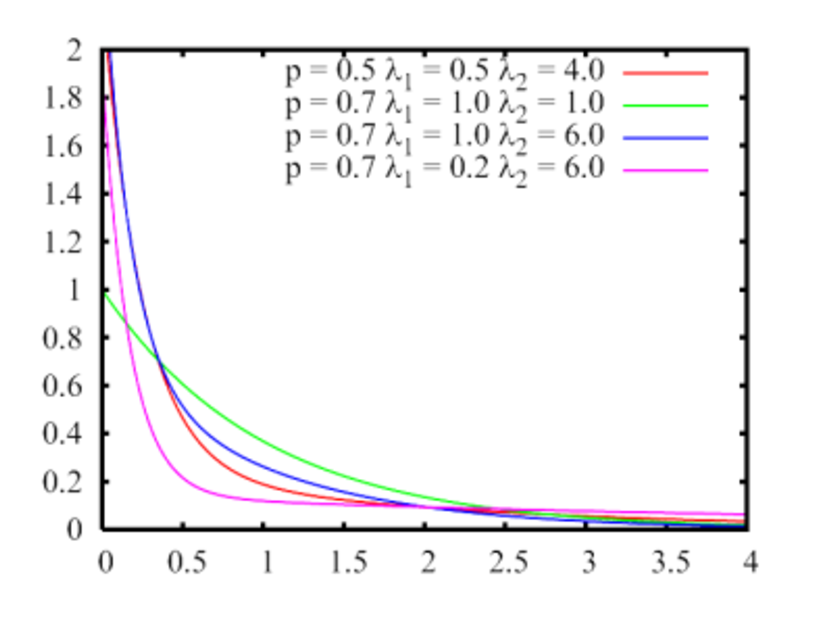
\includegraphics[scale=.5]{img/jsimg/4.8.eps}
    \end{center}
    \caption{Family of hyperexponential density functions}
    \label{fig:famHyper}
\end{figure}

\textbf{\emph{Normal} (norm($\mu,\sigma$)) distribution}\\
The \emph{Normal} distribution is also called Gaussian since its
probability density function is the Gaussian function. It is well
known for its bell-shaped density function.

The two parameters are $\mu$ = location (real number, it is the
\emph{mean} of the distribution), and $\sigma$ = scale (real
number, it is the \emph{standard deviation} of the distribution,
i.e., the square root of the variance). The density is symmetrical
around the mean and the variance. The probability density function
is:
\[
f(x) = \frac{1}{\sqrt{2 \pi \sigma}} \; e^{-\frac{(x-\mu)^2}{2
\sigma^2}}
\]
 The \emph{standard normal distribution} is the normal
distribution with $\mu$ = 0 (mean equal 0) and $\sigma$ = 1
(variance and standard deviation equal 1). A family of normal
density functions is shown in \autoref{fig:famNorm}.
\begin{figure}[htb]
    \begin{center}
        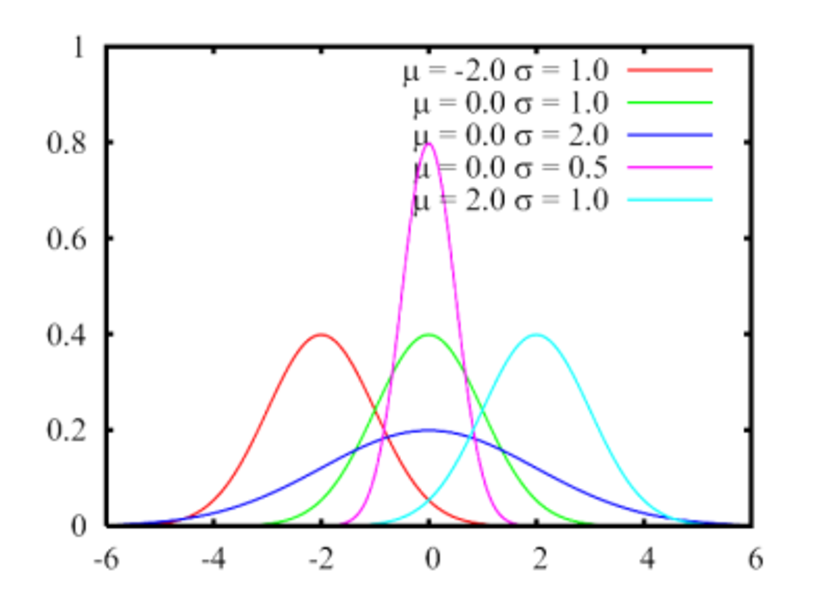
\includegraphics[scale=.5]{img/jsimg/4.9.eps}
    \end{center}
    \caption{Family of normal density functions. The
standard normal density is the green colored.}
    \label{fig:famNorm}
\end{figure}\\

\textbf{\emph{Pareto} (par($\alpha$,k)) distribution}\\
 This
distribution is usually utilized to describe the behavior of
social and economical phenomena (e.g., the distribution of wealth,
where a small portion of the people owns the larger part of the
wealth). It is characterized by the parameters $k>0$, \emph{location}
(real), and $\alpha>0$, \emph{shape} (real). The probability density
function is:
\[ f(x) = \alpha k^\alpha x^{-(\alpha + 1)  }
\]
If \emph{k} and $\alpha$ are provided as input parameters, the simulator
compute the mean  $k \alpha/(\alpha - 1)$ for $k>1$ and the
variance
\[ \frac{\alpha^2 x }{(x-1)^2 (x-2)}
\]
A family of Pareto density functions is shown in
\autoref{fig:famPar}.
\begin{figure}[htb]
    \begin{center}
        \includegraphics[scale=.5]{img/jsimg/4.10.eps}
    \end{center}
    \caption{Family of Pareto density functions.}
    \label{fig:famPar}
\end{figure}\\

\textbf{\emph{Poisson} (poisson($\lambda$)) distribution}\\
The Poisson distribution describes the number of events occurring
in a time interval, when such events are independent of the amount
of time elapsed and they occur at a fix rate. It is a discrete
probability distribution characterized by a single parameter,
$\lambda$, a positive real number, which is the average number of
events in a time interval and its variance. The probability of
having an arrival in a time interval (t, t+$\Delta$t) is $\lambda
\Delta$t+{$o(\Delta t)^2$}, while the probability of more than one
arrival in the same interval is o($\Delta$t).

For large time intervals T, the distribution is near the mean
value, thus the number \emph{n} of arrivals over the interval is
given by \emph{n} = $\lambda$T. The time intervals between two
consecutive events having a Poisson distribution are exponentially
distributed with average value equal to $1/\lambda$. The
probability mass function is:
\[ f(x) = \frac{\lambda^x}{x!} \; e^{-\lambda}
\]
A family of Poisson probability mass functions is shown in
\autoref{fig:famPois}.
\begin{figure}[htb]
    \begin{center}
        \includegraphics[scale=.5]{img/jsimg/4.11.eps}
    \end{center}
    \caption{Family of Poisson probability mass functions.}
    \label{fig:famPois}
\end{figure}\\

\textbf{\emph{Replayer} (replayer("filename")) distribution}\\
When Replayer is chosen, a trace of data provided by the users can
be reused as interarrival times or service times. The file format
should be \texttt{text/binary} with values separated by CR
("\emph{Carriage Return}"). In order to use this user-supplied
file of data, the user should provide in the input window the
absolute path name of the file.\\

\textbf{\emph{Student-T} (studT($\nu$)) distribution}\\
The \emph{T}-distribution, or StudentT distribution, is a continuous
distribution characterized by the single parameter $\nu$, a real
positive number. It is used when the mean of a normally
distributed population must be estimate using only a small sample
size. It is the basis of the Student-\emph{t}'s test that is used to
evaluate the statistical significance of the difference between
two sample means and for the difference between two population
means. It is a special case of the generalized hyperbolic
distribution. The mean is 0 for $\nu>1$ and the variance is
$\nu/(\nu-2)$ for $\nu >$ 2 (infinite otherwise). The probability
density function is:
\[ f(x) = \frac{\Gamma(\frac{\nu+1}{2})}{\sqrt{\nu \pi} \;\;
\Gamma(\frac{\nu}{2}) \;\; (1+\frac{x^2}
{\nu})^\frac{\nu+1}{2}}
\]
where $\Gamma(t)$ is the Eulero function. A family of probability
density functions for a set of $\nu$ values is shown in \autoref{fig:famStut}.
\begin{figure}[htb]
    \begin{center}
        \includegraphics[scale=.5]{img/jsimg/4.12.eps}
    \end{center}
    \caption{Family of \emph{Student-T} density functions.}
    \label{fig:famStut}
\end{figure}\\

\textbf{\emph{Uniform} (U(min,max)) distribution}\\
The \emph{Uniform} distribution, also referred to as Rectangular
distribution due the shape of its density function, describes a
random variable that may assume all the values in the range (min,
max) with the \emph{constant} probability $1/(max-min)$. The
probability is 0 outside the considered range.

The user can either provide the pair (min, max) or the \emph{mean}
$m=(max+min)/2$ and \emph{variance} $c=(max-min)^2 / 12$. Two
uniform density functions are plotted in \autoref{fig:famUnif}.
\begin{figure}[htb]
    \begin{center}
        \includegraphics[scale=.5]{img/jsimg/4.13.eps}
    \end{center}
    \caption{\emph{Uniform} density functions with different range of values.}
    \label{fig:famUnif}
\end{figure}

\section{Performance indices}
\label{perfinde}

The following list include the performance indices that can be obtained from
a simulation run.
\begin{itemize*}
\item \textbf{Queue Length (of a station):} number of customers $N$ at a
station, both waiting and receiving service.

\item \textbf{Queue Time (of a station):} average time spent by the
customers waiting in a station \emph{queue}. It does not include the
Service Time.

\item \textbf{Residence Time (of a station):} total time spent at a
station by a customer, both queueing and receiving service,
considering \emph{all} the visits at the station performed during its complete execution.

\item \textbf{Response Time (of a station):} average time spent in a
station by a customer for a \emph{single} visit (sum of Queue time and
Service time).

\item \textbf{Utilization (of a station):} percentage of time a
station is used (i.e., \emph{busy}) evaluated over all the
simulation run. It ranges from 0 (0\%), when the station is always
\emph{idle}, to a maximum of 1 (100\%), when the station is
constantly \emph{busy} servicing customers for the entire
simulation run. \emph{Queueing stations} may have more than one
server, their number is a parameter to be specified
(\emph{default} is 1). It is important to point out that the
\emph{utilization U} of a queueing station with a \emph{single
server} is given by $U=\lambda S$, and in a station with $m
servers$ the utilization of \emph{any} individual server
is given by $U=\lambda S /m$.\\
In \emph{delay stations}, for consistency with Little's law, the
\emph{utilization} is computed as the \emph{average number of
customers} in the station, and thus it may be \emph{greater than
1}.

\item \textbf{Throughput (of a station):} rate at which customers
departs from a station, i.e., the number of requests completed in
a time unit.

\item \textbf{System Throughput (of the system):} rate at which customers departs
from the system.

\item \textbf{System Response Time (of the system):} average time a customer
spends in the system in order to receive service from the various
stations it visits. It corresponds to the intuitive notion of
response time, as the interval between the submission of a request
and the reception of the response.

\item \textbf{Customer Number (of the system):} average number of
customers in the system. If the index is associated with a closed
class, then it is equal to the number of customers in the class.
\end{itemize*}
Any subset of indices from the above list can be plotted as
model output.
\begin{figure}[htb]
    \begin{center}
        \includegraphics[scale=.5]{img/jsimg/5.1.eps}
    \end{center}
    \caption{The window for the selection of the \texttt{performance indices}.}
    \label{fig:selperfind}
\end{figure}
Each index is associated with a class and a station and will be
computed within the given Confidence Interval and Maximum Relative
Error, both defined on the (0-1) range, by performing the
following steps:\\
\textbf{1.} Select the index you want to add to the model from
this menu:
\begin{figure}[htb]
    \begin{center}
        \includegraphics[scale=.5]{img/jsimg/5.2.eps}
    \end{center}
    \caption{The drop-down list for the selection of the \emph{performance indices}.}
    \label{fig:dropdownlistperfind}
\end{figure}\\
\textbf{2.} Select \texttt{Add Selected Index} and the index will
be added to the
panel. Then the index must be set.\\
\textbf{3.} Select from the \texttt{Class} menu a \texttt{Single
class}, or \texttt{All Classes}, for which the index must be
computed.
\begin{figure}[h!]
    \begin{center}
        \includegraphics[scale=.5]{img/jsimg/5.3.eps}
    \end{center}
    \caption{The drop-down list for the selection of the \texttt{Class}.}
    \label{fig:dropdownlistclass}
\end{figure}\\
\textbf{4.} Select the \emph{Station} for which the index must be
computed from \texttt{Station} menu. In case of system wide
indices, namely, System Throughput and System Response Time, this
option is not available.
\begin{figure}[h!]
    \begin{center}
        \includegraphics[scale=.5]{img/jsimg/5.4.eps}
    \end{center}
    \caption{The drop-down list for the selection of the \texttt{Station}.}
    \label{fig:dropdownliststat}
\end{figure}\\
\textbf{5.} Double click to modify the default values for the
\emph{Confidence Interval} size of the solution and for the
\emph{Max Relative Error} of the greatest sample error, if you
want more/less accurate results.\\
\begin{figure}[!]
    \begin{center}
        \includegraphics[scale=.5]{img/jsimg/5.5.eps}
    \end{center}
    \caption{Definition of the \texttt{Confidence Interval} and
    \texttt{Max.Relative Error}.}
    \label{fig:ConfIntMaxerr}
\end{figure}
\textbf{6.} Repeat these steps for all the indices you want to
include in
the model output.\\

NOTE: Errors in parameter settings will be detected only when the
simulation is started, raising a warning or an error message.

\subsection{Confidence Intervals}
\label{conint} The confidence interval shown at the end of a
simulation run contains the true value of the estimated index with
the selected probability (1-$\alpha$) or, equivalently, if an
experiment is repeated many times, in (1-$\alpha$)*100\% of cases.
Various difficulties in meeting theoretical assumptions can cause
that the real percentage of the confidence intervals containing
the true parameter differs significantly from (1-$\alpha$). The
robustness of the above methods of data collection and analysis is
usually measured by the coverage of confidence intervals, defined
as the frequency with which the intervals (X(n)-$\Delta x$,
X(n)+$\Delta x$) contain the true parameter value $\mu_x$, at a
given confidence level (1-$\alpha$), 0$<\alpha<$1.
\begin{figure}[h]
    \begin{center}
        \includegraphics[scale=.5]{img/jsimg/5.6.eps}
    \end{center}
    \caption{\emph{Confidence intervals} for the correct parameter value $\mu_x$ evaluated
    in 10 runs. The coverage is 80\% since two of them do not include
    the correct value.}
    \label{fig:ConfIntexam}
\end{figure}
The coverage analysis can be applied only to systems with a
theoretical well-known behavior, since the value of $\mu_x$ has to
be known. Any analyzed method must be applied in a statistically
significant number of repeated simulation experiments, usually 200
or more replications, to determine the fraction of experiments
producing the final confidence intervals covering the true mean
value of the estimated parameter.

\subsection{Max Relative Error}
\label{mrerr} Let $x$ be the true value of a quantity and $x_i$ be
the measured or inferred value. The relative error is defined by:
\[ \frac{|\overline{X}(n) - \mu_x|} {|\mu_x|} \;\;\;\; where
\;\;\;\;\overline{X}(n) = \sum_{i=1}^{n}  \frac{x_i}{n}\] where
$\mu_x$ is the mean value.  The relative error is the sum of the
deviations between the sample values and the mean value, divided
for the mean value.

\section{Simulation Parameters}
The \texttt{Define Simulation Parameters} window can be reached
either by selecting \texttt{Simulation Parameters} from the
\texttt{Define} menu or by clicking the \texttt{Define Simulation
Parameters} icon
\includegraphics[scale=.5]{img/jsimg/defineSimulationParameters.eps}
from the toolbar (see \autoref{fig:inistat}).

\begin{figure}[h]
    \begin{center}
        \includegraphics[scale=.5]{img/jsimg/6.2.eps}
    \end{center}
    \caption{Window for the definition of the \texttt{Simulation Parameters}}
    \label{fig:inistat}
\end{figure}

The parameters required by the simulator are:
\begin{itemize*}
\item \textbf{Simulation Seed:} is the number used by the
simulation engine to generate pseudo-random numbers. If you change
the seed, you will obtain a different sequence of pseudo-random
numbers. If a simulation is repeated using the same seed, the same
sequence of pseudo-random numbers will be generated, thus leading
to identical results. The default value is random, which indicates
that the simulation engine will pick a seed of its choice in a
pseudo-random fashion each time it is started; deselect
\texttt{random} and insert a number if you want a custom
simulation.

\item \textbf{Maximum duration (sec):} It represents the maximum
amount of time in seconds that the simulation will run. If the
simulation ends before the maximum duration, the parameter is
ignored and does not affect the results. The \emph{default} value
is \emph{infinite}, deselect it and specify the preferred maximum
time if you do not want the simulation to run for a possibly very
long time. In this case, the simulation stops when the time limit
is reached, although a reliable solution may not be available yet.

\item \textbf{Maximum number of samples:} It is the greatest
number of samples for each index that JSIMgraph collects before
ending the simulation. During a simulation, measurements can be
stopped in case of:\\
- \emph{Success}, if the results have reached the required
Confidence
Interval and the Max Relative Error\\
- \emph{Failure}, if the simulation has analyzed the maximum
number of samples but has not reached the required Confidence
Interval or
Max Relative Error\\
- \emph{Failure}, if timeout occurs before successfully
calculating the final results.

The default value for the maximum number of samples is 500,000;
 you may increase it (for a more accurate simulation) or decrease
it (for a faster simulation).

\item \textbf{Representation Interval (sec):} This is the
granularity at which results are plotted on the screen, i.e., the
time interval before a new point is added to the graphs, as the
simulation proceeds. A large value will make the simulation to
proceed slower, as the graphs are updated less often. Small values
will provide an impression of better "responsiveness" from the
simulation, as graphs are updated more frequently. Animation
checkbox is used to enable or disable queue animation during the
simulation process. \end{itemize*}

{\large{\noindent{\textbf{Initial state of a simulation}}}}

The \emph{Initial state} is the model state at time 0, typically
described by the number of customers in each station at the
beginning of the simulation.

For closed customer classes, all customers are allocated by
\emph{default} to their \emph{reference stations}. You can modify
this allocation, as long as the total number of customers remains
the one defined in the \texttt{Classes} tab. For open customer
classes, it is possible to initialize each station with any
desired number of customers. In \autoref{fig:inistat} the
\emph{initial state} of a model with four stations and two classes
(\emph{ClosedClass} with 3 customers in the \emph{CPU} station and
\emph{Class0} with 10 customers in the \emph{Users} station) is
shown.


\section{What-If Analysis}
\label{whaif}

A What-If Analysis consists of a series of simulations in which
one or more \emph{control} parameters are varied over a specified
range. This allows the observation of system behavior under a
spectrum of conditions, unlike the single simulation run where the
system is observed under a fixed set of parameters. By default the
What-If Analysis is not enabled. It must be activated explicitly
and its parameters should be defined.
\begin{figure}[hbt]
    \begin{center}
        \includegraphics[scale=.5]{img/jsimg/7.1.eps}
    \end{center}
    \caption{The window for \texttt{What-If Analysis} definition.}
    \label{fig:iniwhatif}
\end{figure}

\noindent{\emph{Activating the What-If Analysis}}\\ After
completing the definition of the model and selecting the
\texttt{What-If Analysis} tab, check the \texttt{Enable what-if
analysis} checkbox to activate it.

\noindent{\emph{Selecting the What-If Analysis}}\\ After enabling
the What-If Analysis, it is possible to select the parameter to
control the sequence of simulation runs using the menu of
\autoref{fig:selparwhatif}.
\begin{figure}[hbt]
    \begin{center}
        \includegraphics[scale=.5]{img/jsimg/7.2.eps}
    \end{center}
    \caption{Selection of the parameter for the control
    of a What-If Analysis.}
    \label{fig:selparwhatif}
\end{figure}
When you select a What-If Analysis parameter, the bottom section
of the window of \autoref{fig:iniwhatif} will change depending
upon the parameter. In the right portion a \texttt{Description} is
provided of the selected parameter and of the impact of its
variation. In the left portion the details of the parameter range
(\texttt{From} and \texttt{To} fields) and the number of
executions (\texttt{Steps}) on the range are provided. The set of
modifiable parameters depends upon the number and type of classes
in the model: in a \emph{single class} model, you simply select
the parameters you want to change during simulation while in a
\emph{multiclass} model, you must select the parameter and specify
whether you want to apply the variation to all the classes or just
to one specific class.\\

\noindent{The parameters that may be used to \emph{control the sequence
of executions} in a What-If Analysis are:}
\begin{itemize*}
\item \textbf{Number of Customers:} (only for models with
\textbf{closed} classes)\\
JSIM repeats the simulation changing
the number of customers in each run, starting from the number
inserted in the \texttt{From N} field, to the value inserted in
the \texttt{To N} field. The simulation is repeated
\texttt{Steps(n.of exec.)} number of times.
\begin{figure}[hbt]
    \begin{center}
        \includegraphics[scale=.5]{img/jsimg/7.3.eps}
    \end{center}
    \caption{Selection of the \texttt{Type of population growth} in
    a What-If Analysis.}
    \label{fig:seltypepopg}
\end{figure}
In \autoref{fig:seltypepopg} a What-If Analysis is planned on a
single closed class model. The option \texttt{Increase number of
jobs of one closed class} has been selected. The initial value of
the number of customers is not modifiable from this window, as it
is part of the \texttt{Classes} tab. The final value should be
specified in the field \texttt{To N}. In this case, with a final
value of 20 and 6 Steps, simulations are run for 10, 12, 14, 16,
18 and 20 customers, respectively. Only the customer number in the
class selected in the \texttt{Class} (\emph{ClosedClass}, in the
picture) will be changed. The remaining classes (if they are
present) will keep their initial number of customers. The
simulator control that the sum of the \emph{percentages of jobs}
of the various classes (represented by the components $\beta_i$ of
vector \textbf{$\beta$}) evaluated over the global population $N$
of the model add up to 1, as shown in the \texttt{Population mix}
table on the bottom of the window of \autoref{fig:seltypepopg} in
the simple case of a single class model.

If the \texttt{Increase number of jobs of all closed classes}
option is selected, the overall population is increased keeping
constant the relative proportion of jobs in the various classes,
i.e., the values $\beta_i$ (also referred to as \emph{population
mix}). Because in the JSIM the number of customers in each class
can only be integer numbers, only the population vectors with all
integer components can be considered. Therefore, the actual number
of executions may be
smaller than the one specified.\\
The population mix describes the way the global population is
subdivided between the classes, i.e., the percentage of customers
in each class ($\beta_i$ values) over the total population. The
population mix can be modified extensively selecting the way we
want to change it with the increasing of the global population of
customers: all classes increase proportionally or only one class
increases keeping constant the jobs of the other classes (select
the option \texttt{Increase number of jobs of one closed class} in
this case). Mixed models can be analyzed too. Remember that only
models with closed classes (at least one) will be considered in
this What-If Analysis.

\item \textbf{Arrival Rate:} (only if there are \textbf{open}
classes)

Arrival rate is the frequency at which jobs arrive at a station
during a period of time. Similarly to the number of customers, the
arrival rate can be changed for one specific open class or for all
the open classes in the model.\\ If the option \texttt{Change the
arrival rate of one open class} is selected, the final arrival
rate and the number of steps must be specified.\\
The initial arrival rate is specified in the \texttt{Arrival Rate}
section of the \texttt{Classes} tab and it is not modifiable
here.\\
If the option \texttt{Change arrival rates for all open classes}
is selected, the final value is expressed as a percentage of
increase with respect to the actual value that is applied to the
arrival rates of all the classes.
%\begin{figure}[hbt]
%    \begin{center}
%        \includegraphics[scale=.5]{img/jsimg/7.5.eps}
%    \end{center}
%    \caption{Selection of the final value of \texttt{arrival rate}
%    in a What-if analysis.}
%    \label{fig:selarrrat}
%\end{figure}
\autoref{fig:iniwhatif} shows the settings for a What-If
Analysis of the arrival rate of all the open classes. The
\texttt{To} field is set to 150\%, which means that for each class
the final arrival rate will be 1.5 times greater than the initial
value. 10 runs will be executed with equally spaced (in
percentage) intermediate values of arrival rates.

\item \textbf{Service time:} (for \textbf{all types} of classes)

Service Time is the time required by a customer at each visit of a
station. In this case, besides the final value and the number of
runs to be executed, the station and the customer's class (or all
the classes) whose service time will be varied must be specified.
\begin{figure}[hbt]
    \begin{center}
        \includegraphics[scale=.5]{img/jsimg/7.6.eps}
    \end{center}
    \caption{Selection of the final value of \texttt{service time}
    in a What-If Analysis.}
    \label{fig:selservti}
\end{figure}
\autoref{fig:selservti} shows the settings for a What-If
Analysis of the service time of class \emph{Class1} at station
\emph{Server1}. The service time distribution will not change.
Only its average will be modified to span the range defined by the
initial value (specified in the \texttt{Station Parameters} tab)
and the final value specified here in the \texttt{To} field.

If the \texttt{Change service time of all classes} option is
selected, the range of service time to explore is expressed in
percentage, starting from the initial value specified at model
definition (which is considered as 100\%). The station whose
service time should be modified must be specified.

\item \textbf{Seed:} (for \textbf{all types} of classes)

Unlike the previous cases, where the analysis is performed for a
range of values of one of the model parameters in order to
investigate the system behavior under a variety of conditions, a
What-If Analysis on the seed aims at evaluating the sensitivity of
the simulation engine to numerical conditions, in particular to
the numerical value used by the pseudo-random number algorithm to
generate the sequence of numbers, i.e., the seed.
\begin{figure}[hbt]
    \begin{center}
        \includegraphics[scale=.5]{img/jsimg/7.7.eps}
    \end{center}
    \caption{Selection of the number of repeated executions with
    different \texttt{seeds} in a What-if analysis.}
    \label{fig:selseed}
\end{figure}
The simulation engine uses a pseudo-random number generator to
generate the sequence of values used in each execution. By
changing the seed, a different sequence of values is produced,
thus leading to different numerical results. The first seed is the
one defined in the \texttt{Simulation Parameters} tab. The number
of executions is specified in the panel of \autoref{fig:selseed}
and the simulation engine generates as many pseudo-random seeds to
be used (one for each execution).
\end{itemize*}

\section{Finite Capacity Region (FCR)}
\label{defcap}


A Finite Capacity Region is a region of the model where the number
of customers is controlled. It is possible to define two types of
FC region capacity constraints:
\begin{itemize*}
\item \emph{Shared}: an upper bound for the number of customers
that are in the region, regardless of the classes they belongs to.
\item \emph{Dedicated}: an upper bound for the number of jobs for
a specific customer class in the region
\end{itemize*}
During the simulation the most restrictive constraint is applied.
For example consider a multiclass model with two classes
(\emph{Class1} and \emph{Class2}) with a shared constraint of 100
customers, a dedicated constraint of 30 customers for
\emph{Class1} and no dedicated constraint for \emph{Class2}. If
during the simulation the queue contains 30 customers belonging to
Class1 and 60 customers belonging to \emph{Class2}, an incoming
job of \emph{Class1} will be rejected (as it's dedicated
constraint is violated) while an incoming job of \emph{Class2}
will be accepted (as it will not exceed the shared constraint). If
the initial state was 20 jobs of \emph{Class1} and 80 jobs of
\emph{Class2} an incoming job will always be rejected, despite of
its class, as it would violate the shared constraint.\\

\textbf{How to define a FCR:}\\
\textbf{ 1.}  Select the stations to include in the region with
the mouse: left-click with the mouse and hold it pressed until all
the elements are included. The selected stations are framed with
green dashed lines, as shown in \autoref{fig:selsatfcr}.\\
\begin{figure}[h]
    \begin{center}
        \includegraphics[scale=.5]{img/jsimg/8.1.eps}
    \end{center}
    \caption{Selection of the stations to be included in a FCR.}
    \label{fig:selsatfcr}
\end{figure}
\noindent{\textbf{2.}  Select the icon
\includegraphics[scale=.5]{img/jsimg/addStationToNFCR}  and
the Finite Capacity Region will
appear with a blue background, see \autoref{fig:selfcrblueback}}.\\
\begin{figure}[h]
    \begin{center}
        \includegraphics[scale=.5]{img/jsimg/8.2.eps}
    \end{center}
    \caption{The area with the blue background is the FRC.}
    \label{fig:selfcrblueback}
\end{figure}
\textbf{3.}  Double click on \texttt{FCRegion} to set the
properties. The properties panel will appear,
\autoref{fig:fcrdefprop}.
\begin{figure}[h!]
    \begin{center}
        \includegraphics[scale=.5]{img/jsimg/8.3.eps}
    \end{center}
    \caption{Window for the definition of the FCRegion properties.}
    \label{fig:fcrdefprop}
\end{figure}

\textbf{Global Properties}\\
 \emph{Region Name}: the name of the region
created\\
\emph{Region Capacity}: max number of customers that can be in the
region. Enable Infinite if you don't want a bound.\\

\textbf{Class Specific Properties}\\
 In the bottom part of the
panel the class specific properties can be defined. Here you can
define each class capacity as infinite or as defined, in same way
stated above for FCR capacity, and choose the dropping property of
the class.

\emph{Capacity}: maximum number of customers of that class into
the FCR.\\
\emph{Drop}: when the FCR is busy, and Drop is "false", the
incoming jobs are not dropped but are put into a temporary queue,
until the FCR can accept them, otherwise they are dropped from the
network.

\section{Defining Network Topology}
\label{defnettop}
To define a new model select \texttt{New} from \texttt{File} menu or
click the icon
\includegraphics[scale=.5]{img/jsimg/new.eps} and draw the
network topology.\\

\noindent \textbf{Selecting the stations}\\ From the second
toolbar (\autoref{fig:statdraw}), select a station and click on
the model panel to insert it (drag and drop). The available
stations
are:\\
\begin{figure}[h!]
    \begin{center}
        \includegraphics[scale=.5]{img/jsimg/8.4.eps}
    \end{center}
    \caption{The toolbar for the selection of the stations to be
    inserted in the network.}
    \label{fig:statdraw}
\end{figure}\\

\noindent{\includegraphics[scale=.5]{img/jsimg/insertSource}
Insert a source
station}\\
\includegraphics[scale=.5]{img/jsimg/insertSink} Insert a sink station\\
\includegraphics[scale=.5]{img/jsimg/insertRouter} Insert a routing
station\\
\includegraphics[scale=.5]{img/jsimg/insertDelay} Insert a delay station\\
\includegraphics[scale=.5]{img/jsimg/insertServer} Insert a queueing station\\
\includegraphics[scale=.5]{img/jsimg/insertFork} Insert a fork node\\
\includegraphics[scale=.5]{img/jsimg/insertJoin}  Insert a join node\\
\includegraphics[scale=.5]{img/jsimg/logger}  Insert a logger station\\
\includegraphics[scale=.5]{img/jsimg/addStationToNFCR}  Add selected stations to a new Finite Capacity
Region\\
To rotate a component press the
\includegraphics[scale=.5]{img/jsimg/rotate} button.
To optimize the final layout of the network press the Press the
\includegraphics[scale=.5]{img/jsimg/optimizeGraph} button.

\textbf{Connecting two elements}\\
To link two stations of the model:

1. Select the icon
\includegraphics[scale=.5]{img/jsimg/connect}

2. Select and hold the mouse pressed from one station to the other
station to which you want to connect to.


\subsection{Source Station}
\label{sstatlab} \textbf{Setting station properties}\\ \emph{Open
classes} are characterized by an infinite stream of jobs that can
enter the system. Source stations are used to generate customers
in the model. The interarrival time of the customers of each class
should be defined as a parameter of the class. The routing
strategy defines the first station a newly created customer will
visit. Only open class customers can be routed from source
stations.\\

\noindent{\textbf{Setting or changing the properties}}\\ Double
click on the station icon to open the properties panel of
\autoref{fig:statprop}. There is only one section:
\texttt{Routing Section}.\\
\begin{figure}[htb]
    \begin{center}
        \includegraphics[scale=.5]{img/jsimg/8.5.eps}
    \end{center}
    \caption{Window for the \texttt{Editing} of the properties of a
    \texttt{Source} station.}
    \label{fig:statprop}
\end{figure}

\noindent \textbf{Routing Section}\\ In the routing section, for
each class, the generated customers are routed to the devices
connected to the analyzed station according to various routing
strategies. The following algorithms are available:
\begin{itemize*}
\item \textbf{Random:} Customers are routed randomly to one of the
stations connected in output to the considered station. The
outgoing links are selected with the same probability.
\autoref{fig:routrand} illustrates the routing strategy with 3 output
links. For each link the probability to be selected is 1/3.
\begin{figure}[htb]
    \begin{center}
        \includegraphics[scale=.5]{img/jsimg/8.7.eps}
    \end{center}
    \caption{Routing with \emph{Random} algorithm.}
    \label{fig:routrand}
\end{figure}

\item \textbf{Round Robin:} Customers are cyclically routed to the
outgoing links according to a circular routing. As shown in
\autoref{fig:routrr}, the first customer is sent to the top
station, the second customer is sent to the central station, and
the third customers is sent to the bottom station. The next
customers would be sent to the top station again, and so on.
\begin{figure}[htb]
    \begin{center}
        \includegraphics[scale=.5]{img/jsimg/8.8.eps}
    \end{center}
    \caption{Routing with \emph{Round Robin} algorithm.}
    \label{fig:routrr}
\end{figure}

\item \textbf{Probabilities:} The routing probability for each
outgoing link must be defined. The sum of all probabilities must
be equal 1 (\autoref{fig:defprobw} and \autoref{fig:routexe}). If the
values provided do not satisfy the constraint, JSIM automatically
normalizes the values before the simulation starts. The
probability for each output link may be set in the panel on the
bottom right of the window shown in \autoref{fig:statprop}.
\begin{figure}[h!]
    \begin{center}
        \includegraphics[scale=.5]{img/jsimg/8.9.eps}
    \end{center}
    \caption{Definition of the probability of the outgoing links.}
    \label{fig:defprobw}
\end{figure}
\begin{figure}[h!]
    \begin{center}
        \includegraphics[scale=.5]{img/jsimg/8.10.eps}
    \end{center}
    \caption{Routing according to the \emph{Probability} algorithm.}
    \label{fig:routexe}
\end{figure}
\item \textbf{Join the Shortest Queue, JSQ}: (sometimes referred
to as \emph{Shortest Queue Length}) Each customer is routed to the
station connected in output that has the \emph{smallest} number of
customers either in queue and in service at the time the customer
leaves the routing station. \autoref{fig:routsql} shows a case
where the number of customers (in queue and in service) at the
devices are 3, 2, and 1 job, respectively, from top to bottom. The
exiting customer will be routed to the bottom station, since its
queue is the shortest (1 customer).
\begin{figure}[htb]
    \begin{center}
        \includegraphics[scale=.5]{img/jsimg/8.11.eps}
    \end{center}
    \caption{Routing according to the \emph{Join the Shortest Queue} algorithm.}
    \label{fig:routsql}
\end{figure}
\item \textbf{Shortest Response time:} Customers are sent to the
station where the average response time for the job's class is the
smallest at the moment a customer leaves the routing station.
\autoref{fig:routstrespt} shows that at the time of routing,
the middle station has the smallest average response time, R, so
the customer will be sent to it.
\begin{figure}[htb]
    \begin{center}
        \includegraphics[scale=.5]{img/jsimg/8.12.eps}
    \end{center}
    \caption{Routing according to the \emph{Shortest Response Time} algorithm.}
    \label{fig:routstrespt}
\end{figure}

\item \textbf{Least Utilization:} The destination station is
chosen as the one with the smallest average utilization at the
time routing is performed. In the example, shown in
\autoref{fig:routleasut} depicted in the picture, the top station
is the least utilized, so it will receive the next customer to
leave the blue station.
\begin{figure}[htb]
    \begin{center}
        \includegraphics[scale=.5]{img/jsimg/8.13.eps}
    \end{center}
    \caption{Routing according to the \emph{Least utilization} algorithm.}
    \label{fig:routleasut}
\end{figure}

\item \textbf{Fastest Service:} A customer is routed to the device
with the smallest average service time, S, for the job's class. In
\autoref{fig:routfastserv} the exiting customer will be routed to
the top station since its service time is the minimum among the
three.
\begin{figure}[htb]
    \begin{center}
        \includegraphics[scale=.5]{img/jsimg/8.14.eps}
    \end{center}
    \caption{Routing according to the \emph{Fastest Service}
    algorithm.}
    \label{fig:routfastserv}
\end{figure}
\end{itemize*}

\subsection{Sink Station} Open class customers leave the
system once they have received all the services they need. Sink
stations are used to model customers leaving the system, as they
enter the sink station but do not ever leave it. Sink stations
have no parameters, only incoming connections from one or more
stations, depending upon the model.

\subsection{Delay Station}
\label{dstat} Customers that arrive at this
station are delayed for the amount of time that defines the
station service time. They do not experience any queuing, since a
delay station is modelled as a station with an infinite number of
servers with the same service time. Thus response time of delay
stations is equal to the service time, $R_i = S_i$. Furthermore,
the queue length corresponds in this case to the number of
customers receiving service since there is no waiting: $Q_i = R_i
X_i = S_i X_i = U_i$. \emph{In delay stations}, for consistency
with Little's law, the \emph{utilization} is computed as the
\emph{average number of customers} in the station, and thus it may
be \emph{greater than 1}.

Delay stations are used when it is necessary to produce some known
average delay. A common application of delay stations is to model
transmission time (download, upload, ...) of large amounts of data
over a network (Internet, lans, ...) or to model users think time
at the browsers.\\

\noindent{\textbf{Setting or changing the properties}}\\ Double
click on the icon representing the delay station to see the
property panel.\\
\begin{figure}[htb]
    \begin{center}
        \includegraphics[scale=.5]{img/jsimg/8.15.eps}
    \end{center}
    \caption{Windows for the editing of \texttt{delay properties}.}
    \label{fig:editdprop}
\end{figure}

\noindent{\textbf{Service Section}}\\ Delay stations are infinite
servers with the same service time characteristics; the service
time distribution should be defined. The infinite numbers of
servers provide the same  average response time for all jobs, as
no job waits in queue for service. The load \emph{dependent} or
\emph{independent} characteristic of the service time must be
specified for each class of customers through the menus of
\autoref{fig:editdprop} and \autoref{fig:selloaddep}.
\begin{figure}[htb]
    \begin{center}
        \includegraphics[scale=.5]{img/jsimg/8.16.eps}
    \end{center}
    \caption{Selecting load dependency.}
    \label{fig:selloaddep}
\end{figure}

\begin{itemize*}
\item \textbf{Load Independent}: A load independent service
indicates that, regardless of the number of customers that are in
the station, the system will serve all the customers following a
fixed policy modelled by the chosen statistical distribution. To
choose the Distribution press the \texttt{Edit} button and insert
all the parameters from the window of \autoref{fig:cldistrw}.
\begin{figure}[htb]
    \begin{center}
        \includegraphics[scale=.5]{img/jsimg/8.17.eps}
    \end{center}
    \caption{Editing of the parameters of a \texttt{distribution}.}
    \label{fig:cldistrw}
\end{figure}

The following service time distributions (see \autoref{distns})
are supported: \emph{Burst (General), Constant, Erlang,
Exponential, Gamma, Hyperexponential, Normal, Pareto, Poisson,
Student-T, Uniform}.

\item \textbf{Load Dependent}: A load dependent service time
indicates that the amount of time the server spends with each
customer depends upon the current number of customers in the
station. A set of intervals for the number for jobs in the station
is specified, either by adding one range at a time via the
\texttt{Add Range} button or by specifying the total number at
once. For each range its lower (\texttt{From} button) value must
be specified. Automatically its upper value (\texttt{To} field) is
computed. Each range of values can be associated with different
service times, distribution, mean and coefficient of variation, or
a subset of them. To set the parameters of a Load Dependent
service time, click the \texttt{Edit} button to edit the Service
Time Distribution. The panel of \autoref{fig:ldservstrat}
appears, then specify the parameters for each range.\\
\begin{figure}[htb]
    \begin{center}
        \includegraphics[scale=.5]{img/jsimg/8.18.eps}
    \end{center}
    \caption{Window for editing a \texttt{load dependent} service strategy.}
    \label{fig:ldservstrat}
\end{figure}
For each range of the number of customers the following parameters
must be described: \begin{itemize*} \item \textbf{Distribution}:
you can choose among Burst (General), Burst (MMPP2), Pareto,
Erlang, Exponential, Hyperexponential, Poisson, Uniform, Constant,
Gamma and Normal distribution. \item \textbf{Mean}: the mean value
of each distribution is specified in the "Mean" form by double
clicking on it. Insert a number or an arithmetic expression that
will be evaluated with JFEP - Java Fast Expression Parser. For a
complete list of the command supported by JFEP you can read the
\texttt{Help} tab or see the JFEP web site at
http://jfep.sourceforge.net/ \item \textbf{c}: The coefficient of
variation of each distribution (when $c$ exists) can be specified
by double clicking on the $c$ form. For example, in
\autoref{fig:ldservstrat} two distributions are defined: when
there is only one customer in the station the service times are
generated according to an Erlang distribution with \emph{mean=1}
and \emph{c=0.5}. For any number of customers greater than 1 in
the station, the service times are generated according to an
Hyperexponential distribution with \emph{mean=1} and $c=1.19$.
\end{itemize*}
\noindent To delete a range click on the \emph{delete} icon
\includegraphics[scale=.5]{img/jsim/delete.eps}
at the end of the correspondent row.

\end{itemize*}

\noindent{\textbf{Routing Section}}\\ In the routing section, for
every class defined, you can decide how the completed jobs are
routed to the other devices connected to station for which the
routing strategy is defined.
\begin{figure}[htb]
    \begin{center}
        \includegraphics[scale=.5]{img/jsimg/8.19.eps}
    \end{center}
    \caption{Selecting the \texttt{Routing Strategy}.}
    \label{fig:selroutstrate}
\end{figure}
For each class, the user should select the algorithm you want to
use for outgoing connections. The following algorithms are available:\\
- Random\\ - Round Robin\\ - Probabilities\\ - Join the Shortest Queue\\
- Shortest Response time\\ - Least Utilization\\ - Fastest Service.\\
To know details about these algorithms, please refer to
\autoref{sstatlab} of \emph{Source Station}.

\subsection{Fork Station}
\label{fstlab}
 A Fork station is a station where jobs
are split into tasks. No service is provided; therefore there is
no service time specification. Tasks are then routed along the
Fork station outgoing links (see \autoref{fig:forkprop}).\\
\begin{figure}[htb]
    \begin{center}
        \includegraphics[scale=.5]{img/jsimg/8.23.eps}
    \end{center}
    \caption{The Fork and Join stations.}
    \label{fig:forkprop}
\end{figure}
Unlike classical queueing theory fork-join queues, a JSIM Fork
station is not associated with a join station automatically. Any
combination of queueing stations, Finite Capacity Regions,
fork-join, routing stations, loggers, etc., is possible after a
Fork station. This feature allows the modelling of very general
parallel behaviors, of which the traditional Fork-Join one is a
special case. In JSIM the classical queueing theory fork-join
queue behavior is obtained by connecting the Fork station to as
many queueing stations as the degree of parallelism requested,
with one task per outgoing link. Each queueing station is then
connected to a Join station, where the job is recomposed.\\ A Fork
station is characterized by the \emph{forking degree}, i.e., the
number of tasks routed on each one of its outgoing links, and the
\emph{capacity}, i.e., the maximum number of jobs that can be
served by the station simultaneously. Therefore, the number of
\emph{sibling tasks} a job is split into is given by the product
of the number of outgoing links from the Fork station times the
forking degree. Note that a finite station capacity makes sense
only when there is a Join station downstream from the Fork station
that can recompose the split jobs. Otherwise, inconsistencies in
the model and subsequent simulation error, such as out-of-memory,
may occur. No automatic checks to identify such critical
conditions have been implemented since it may happen that users
are required to simulate special conditions purposely. Both the
forking degree and the capacity are section parameters to be
specified in the model. As an example, a Fork station with forking
degree 1, connected to three queueing stations, would split a job
into 3 sibling tasks (this is a traditional Fork-Join like
behavior). If no Join station is connected to any of the three
Servers, a warning message is displayed since the model could
quickly saturate due to the extra load (3 more customers) created
in addition to each job entering
the Fork station.\\

\noindent{\textbf{Set or change of properties}}\\
 The station has two
sections: \texttt{Fork Section} and \texttt{Queue Section}.

\noindent \textbf{Fork Section}: In this section the user can
define the station \emph{forking degree}, i.e., the number of
tasks created for each job arriving at the fork station, and its
\emph{capacity}, i.e., the maximum number of jobs that can be in a
fork-join section (when a join is present):
\begin{figure}[htb]
    \begin{center}
        \includegraphics[scale=.5]{img/jsimg/8.21.eps}
    \end{center}
    \caption{Setting of the \texttt{Fork degree} and the \texttt{Fork capacity}.}
    \label{fig:forkdegcap}
\end{figure}
\begin{itemize*}
\item \textbf{Forking degree}: It is the number of tasks that are
routed on each outgoing link of the fork station. Therefore, each
customer is split into \emph{(forking degree)}x\emph{(number of
outgoing links)} tasks. By \emph{default} the forking degree is 1,
it can be modified as shown in \autoref{fig:forkdegcap}. \item
\textbf{Capacity:} It is the maximum number of customers (jobs)
that can be served by a Fork-Join section simultaneously. It makes
sense only if there is a Join station matching the Fork one. It
can be \emph{finite}, in this case when the limit is reached the
jobs wait in the queue of the Fork station. A job is removed from
the queue and serviced (i.e., split into tasks) when a job is
recomposed at the matching Join station and leaves it. Capacity is
defined using the form shown in \autoref{fig:forkpropwind}, after
checking the \texttt{Finite capacity...} box.
\end{itemize*}

\noindent \textbf{Queue Section}\\
 The Queue section allows the
specification of the queueing \emph{capacity} (finite or infinite)
and \emph{policy}. Different classes of customers may have
different policies associated with
them.\\
\begin{figure}[htb]
    \begin{center}
        \includegraphics[scale=.6]{img/jsimg/8.22.eps}
    \end{center}
    \caption{Window for the editing of the \texttt{Fork properties}.}
    \label{fig:forkpropwind}
\end{figure}
\begin{itemize*}
\item \textbf{Capacity:} a station can accept any customer and let
them wait in queue, in which case its capacity is considered
infinite, or it can only accept a finite number of customers. In
this case its capacity is finite, the max number of customers is
to be specified in the field \texttt{length}.

\item \textbf{Queue policy:} it is the algorithm used to decide
which customer to serve next. A variety of factors can contribute
to the order in which customers are served, such as arrival order,
priorities associated with a class, the amount of service already
provided to customers, etc. In JSIM queuing disciplines based on
arrival order and priority are the only available, namely:
\begin{itemize*}
\item \textbf{FCFS:} under the First Come First Served queuing
discipline, customers are served in the order in which they arrive
at the station. If the model is exported to MVA, the following
constraint is enforced in the exported model. Since all customer
classes must have the same average service time at a FCFS station,
the total number of visits to the station ($V_c,k$) is adjusted in
order to comply with the constraint and at the same time allow for
distinct service demands ($D_c,k$). \item \textbf{FCFS
(Priority)}: under this policy, customers are ordered according to
their arrival time but customers with higher priority jump ahead
of customers with lower priority (conventionally a small priority
number = low priority). Customers with the same priority are
served FCFS. \item \textbf{LCFS:} under the Last Come First Served
queuing discipline, an arriving job jumps ahead of the queue and
will be served first, unless other jobs arrive before the one
currently in service finishes. The LCFS discipline implemented in
JSIM is not the preemptive-resume type. \item \textbf{LCFS
(Priority):} under this policy, the next customer to be served is
one with the highest priority (conventionally a small priority
number = low priority), so an arriving customer can only jump
ahead of the queue of the other jobs with the equal or smaller
priority. Customers with the same priority are served LCFS.
\end{itemize*}
\item \textbf{Drop Rule:} it is not active when infinite capacity
is selected. For each class you can select a rule to apply when a
customer cannot enter a station since the max number of customers
allowed is reached.
\end{itemize*}

\subsection{Join Station}
 \emph{Join} stations are complementary to fork
stations (see \autoref{fig:forkprop}). In classical queueing
network theory, a task arrives at a join station from the
corresponding Fork station.\\

In JSIM, a Join station may have incoming links from stations
other than the corresponding Fork one. A \emph{Join} station has
\emph{no service time}, as it is only used to recombine the tasks
a job had been previously split into and then route the job to
some other station(s). When a task arrives at a join station, it
waits until all its sibling tasks have arrived. At this time, the
original job is recomposed and routed to the next station. If a
job arrives from a station other than the corresponding Fork,
i.e., a job that was not split, it is simply routed to the next
station. In this
case the Join station operates as a routing station\\

\noindent \textbf{ Set or change of properties}\\ It has only the
\texttt{Routing} section.\\
\begin{figure}[htb]
    \begin{center}
        \includegraphics[scale=.5]{img/jsimg/8.24.eps}
    \end{center}
    \caption{Editing of the \texttt{Routing Strategy}.}
    \label{fig:edjprop}
\end{figure}

\noindent \textbf{Routing Section:}\\ In the routing section, for each class
defined, you can decide how the completed jobs are routed to the
other devices connected to the station for which the routing
strategy is defined.
%\begin{figure}[htb]
%    \begin{center}
%        \includegraphics[scale=.5]{img/jsimg/8.25.eps}
%    \end{center}
%    \caption{Selecting the \texttt{Routing strategy}.}
%    \label{fig:selroutstrat}
%\end{figure}
For each class, the user should select the algorithm applied to
determine the path followed by the outgoing customers.
The following algorithms are available:\\
- Random\\  - Round Robin\\ - Probabilities\\   - Join the Shortest Queue JSQ\\
- Shortest Response time\\ - Least Utilization\\  - Fastest Service.\\

\noindent To know details about these algorithms, please refer to the
\autoref{sstatlab} \emph{Source Station}.


\subsection{Routing Station}
 A \emph{routing} station is a dummy
station, with service time equal 0, which is used to create more
sophisticated routing strategies by sending customers through one
or more such stations. For example, if we want that two thirds of
the incoming traffic at station Z to be randomly routed to either
station A or B or the remaining third to go either to station C or
D, depending on the shortest queue at the two stations, we could
implement the following. Add a routing station, Y, to the output
of Z station and define random routing for the three stations
connected in output (namely, A, B, Y). Then connect Y to C and D
and define
shortest queue routing JSQ for C and D.\\
\begin{figure}[htb]
    \begin{center}
        \includegraphics[scale=.5]{img/jsimg/8.26.eps}
    \end{center}
    \caption{The \texttt{Routing Station}.}
    \label{fig:routstat}
\end{figure}

\noindent \textbf{Set or change of properties}\\ With a double click on the
routing station icon, the \texttt{Editing Routing Station
Properties} window is shown (see \autoref{fig:edjprop}).
%\begin{figure}[htb]
%    \begin{center}
%        \includegraphics[scale=.5]{img/jsimg/8.27.eps}
%    \end{center}
%    \caption{Window for the editing of \texttt{Routing station properties}.}
%    \label{fig:rstprop}
%\end{figure}
It has only one tab \texttt{Routing Section}.\\

\noindent \textbf{Routing Section:}\\ In the routing section, for
each class, you can decide how the completed jobs are routed to
the other devices connected to the considered station.
%\begin{figure}[htb]
%    \begin{center}
%        \includegraphics[scale=.5]{img/jsimg/8.28.eps}
%    \end{center}
%    \caption{Window for the selection of the \texttt{Routing strategy}.}
%    \label{fig:rostrat}
%\end{figure}
For each class, the user should select the algorithm applied to
determine the path followed by the outgoing customers.
The following algorithms are available:\\
- Random\\  - Round Robin\\ - Probabilities\\   - Join the Shortest Queue JSQ\\
- Shortest Response time\\ - Least Utilization\\  - Fastest Service.\\

\noindent To know details about these algorithms, please refer to the
\autoref{sstatlab} \emph{Source Station}.

\subsection{Queueing Station}
 The \emph{Queueing Station} is one of the most
important components in a queueing network model. A queueing
station consists of two main components: a \texttt{queue} and a
\texttt{server} (one or more) to execute the requests. If all the
servers of the station are busy when a new customer arrives at the
station, the arriving customer join the queue and waits its turn
to receive service from the first idle server. The queueing
discipline determine which customer is served next when a server
becomes free. The response time at queueing stations includes
service time and queueing time. Queueing stations may have more
than one server, their number is a parameter to be specified
(\emph{default} is 1).
\begin{figure}[htb]
    \begin{center}
        \includegraphics[scale=.5]{img/jsimg/8.29.eps}
    \end{center}
    \caption{The \texttt{Queueing Station} icon.}
    \label{fig:questat}
\end{figure}
It is important to point out that the \emph{utilization U} of a
queueing station with a \emph{single server} (i.e., the fraction
of time in which the server is busy) is given by $U=\lambda S$,
and in a station with $m servers$ the utilization of \emph{any}
individual server
is given by $U=\lambda S /m$.\\

\noindent \textbf{Set or change of the properties}\\
Double click on the \texttt{Queueing Station} icon and the
\texttt{Editing Server
Properties} window will open (see \autoref{fig:questatset}).\\
\begin{figure}[htb]
    \begin{center}
        \includegraphics[scale=.5]{img/jsimg/8.30.eps}
    \end{center}
    \caption{Window for editing the \texttt{Queueing (server) Station} properties.}
    \label{fig:questatset}
\end{figure}
\texttt{Station name} is the name of the station that the user
like to assign. There are three tabs: \texttt{Queue Section,
Service Section} and \texttt{Routing Section}.\\

\noindent \textbf{Queue Section}\\
Please refer to \emph{Queue Section} of \autoref{fstlab} \emph{Fork Station}\\


\noindent{\textbf{Service Section}}\\
The service time
distribution and the number of servers (\emph{default} is 1)
should be defined. The load \emph{dependent} or \emph{independent}
characteristic of the service times must be specified for each
class of customers through the menus of \autoref{fig:editdprop} and
\autoref{fig:selloaddep}.\\
Please refer to \emph{Service Section} of \autoref{dstat} \emph{Delay Station}.\\



\noindent{\textbf{Routing Section}}\\ In the routing section, for
each class of customers, you can decide the path followed by the
completed jobs are routed to the devices connected to station for
which the routing strategy is defined.
%\begin{figure}[htb]
%    \begin{center}
%        \includegraphics[scale=.5]{img/jsimg/8.19.eps}
%    \end{center}
%    \caption{Selecting the \texttt{Routing Strategy}.}
%    \label{fig:selroutstrate}
%\end{figure}
For each class, the user should select the algorithm you want to
use in order to determine the outgoing connection followed by a
customer.
The following algorithms are available:\\
- Random\\ - Round Robin\\ - Probabilities\\ - Join the Shortest Queue - JSQ\\
- Shortest Response Time\\ - Least Utilization\\ - Fastest Service.\\
To know details about these algorithms, please refer to the
\texttt{Routing Section} of \autoref{sstatlab}-\emph{Source
Station}.
%\begin{figure}[htb]
%    \begin{center}
%        \includegraphics[scale=.5]{img/jsimg/8.32.eps}
%    \end{center}
%    \caption{Window for edit a \texttt{Distribution} parameters.}
%    \label{fig:distrubpar}
%\end{figure}

%\begin{figure}[htb]
%    \begin{center}
%        \includegraphics[scale=.5]{img/jsimg/8.33.eps}
%    \end{center}
%    \caption{Definition of the service times for load dependent stations.}
%    \label{fig:distrubpar}
%\end{figure}


\subsection{Logger station}
\label{logsta} A logging station (i.e., \emph{logger}) reads information
flowing through it and writes it to a file.   In the simplest way,
it is a tool to understand and debug the traffic flow moving
through the interesting part(s) of the model. Place the logger
station into the model, choose the parameters, and trace the data
as it passes through the model.\\

\noindent \textbf{Set or change of the properties}\\
Double click on the \texttt{Logger Station} icon
\includegraphics[scale=.5]{img/jsimg/logger}
to open the \texttt{Editing Logger Properties} station's
configuration dialog (see \autoref{fig:deditlogg}). There are two
sections:
\texttt{Logger Section} and \texttt{Routing Section}.\\
\begin{figure}[htb]
    \begin{center}
        \includegraphics[scale=.8]{img/jsimg/logger_editFull_sm.eps}
    \end{center}
    \caption{Window for the \texttt{Logger Station} configuration.}
    \label{fig:deditlogg}
\end{figure}

\noindent{\textbf{Logger Section}}\\
The configuration properties of the \texttt{Logger Section} are:
\begin{itemize*} \item \textbf{Logging Options:}
\begin{itemize*} \item   The Logfile's name to use, either individual or merged
(Logger0.csv or global.csv, respectively). \item The information
to log (fields): Logger Name, Job Arrival Time (simulation units),
unique Job ID, defined Class ID, Interarrival time of same class,
Interarrival time of any class. These fields are found in the next
section. \end{itemize*} \item \textbf{Logfile Options:}
\begin{itemize*} \item Browse button: allows changing the directory where
logfiles are stored. \item Overwrite method to use when the
logfile exists, and a new simulation needs to overwrite the file.
Replace overwrites the file, append adds data to the end of the
file. \item Delimiter chooses the character to separate between.
\end{itemize*}
\item \textbf{Status} displays the path and file-status of the
logfile that is going to be written.
\end{itemize*}

As messages flow through the Logger from one station to another,
the following information can be logged:
\begin{itemize*} \item \texttt{Logger Name}, the name of the logger
where the message occured (e.g., \emph{Logger0}) \item \texttt{Job
arrival time}, this timestamp marks the current simulation time
from start of simulation (not seconds) \item \texttt{Job ID}, the
auto-generated unique sequence number of the message (e.g.
1,2,3...). \item \texttt{Class ID}, the name of \emph{customer
class} of message (e.g., \emph{Class0}) \item \texttt{Interarrival
time (same class)}, is a time difference between customer of the
same class that passes through the logger \item
\texttt{Interarrival time (any class)}, is a time difference
between customers of any class that passes through the logger.
\end{itemize*}

Once a \emph{Logger} is configured, running a simulation produces
a logfile with the chosen fields. An example
of logfile output is:\\
\texttt{LOGGERNAME;TIMESTAMP;JOBID;JOBCLASS;TIMEELAPSED\_SAMECLASS;
TIMEELAPSED\_ANYCLASS\\ Logger0;0.199;1;Class0;0.000;0.199\\
Logger0;0.559;2;Class0;0.341;0.341}\\

\noindent{\textbf{Routing Section}}\\
For each class of customers, the user should select the algorithm
that want to apply in order to determine the outgoing connection
(i.e., the routing strategy) followed by a customer  that
completed its service in the current station.
The following algorithms are available:\\
- Random\\ - Round Robin\\ - Probabilities\\ - Join the Shortest Queue - JSQ\\
- Shortest Response Time\\ - Least Utilization\\ - Fastest Service.\\
To know details about these algorithms, please refer to the
\texttt{Routing Section} of \autoref{sstatlab}-\emph{Source
Station}.


\section{Modification of the Parameters}
\label{modifpa}

\subsection{Modifying Simulation Parameters}
To modify the simulation or initial state parameters , the user
has to select \texttt{Simulation Parameters} (icon
\includegraphics[scale=.4]{img/jsimg/defineSimulationParameters.eps})
from the \texttt{Define} menu and change the values. From
\texttt{Simulation Parameters} the user can:
\begin{enumerate*} \item change the \emph{Initial state}, i.e., the location
of the customers at the beginning of the simulation \item change
or confirm the \emph{seed} of the random number algorithm in order
to have different run of the simulation \item change the maximum
number of \emph{samples} \item change the time interval used in
the graphical representation of the indices \item change or
confirm the maximum \emph{duration} of the simulation.
\end{enumerate*}

\noindent For more details about these parameters see the Section
\texttt{Simulation Parameters} of \autoref{modefpara}.

\subsection{Modifying station parameters}
 To modify the
parameters of a station select the icon
\includegraphics[scale=.5]{img/jsimg/select} and double
click on the station to modify. The properties panel of a station
will be opened and the modifications could be applied.\\
To see a complete list of properties of each station see
\autoref{defnettop} \emph{Defining Network Topology}.

\subsection{Modifying the default values of parameters}
\label{modefpara} The simulator default settings for \emph{Class,
Station, Simulation,} and \emph{Finite Capacity Region} parameters
can be changed from the \texttt{Define} menu in the menu bar. At
first the user need to select \texttt{Default parameters} from the
\texttt{Define} menu.
\begin{figure}[htb]
    \begin{center}
        \includegraphics[scale=.5]{img/jsimg/9.1.eps}
    \end{center}
    \caption{Selection of the \texttt{Default parameters} from the
    \texttt{Define} menu.}
    \label{fig:seldepardef}
\end{figure}
Alternatively, the user can select the
\includegraphics[scale=.5]{img/jsimg/defineDefaults} (\texttt{Define
default values} of model parameters) button. In JSIMgraph all the
parameters have default values. Such values can be changed to suit
the user's most common modelling activities. The default values of
\emph{Class, Station, Simulation, Finite Capacity Region (FCR)}
and their possible modifications are described in the
following sections.\\

\noindent \textbf{Class Parameters}\\
These settings define the default values of class parameters
assigned to a new class (see \autoref{fig:clparam}).
\begin{figure}[htb]
    \begin{center}
        \includegraphics[scale=.5]{img/jsimg/9.2.eps}
    \end{center}
    \caption{The \texttt{Class parameters} modification window.}
    \label{fig:clparam}
\end{figure}
\begin{itemize*}
\item \emph{Name:} The default name for each newly created class
of customers is "\emph{Class}", followed by a progressive integer,
starting from 1, indicating how many classes you have created so
far. It can be set to any alphanumerical string, which
automatically will be followed by the same numbering scheme. \item
\emph{Type:} The default class type is "\emph{Closed}". If open
classes are used more often, you may want to change to Open as
default, so as to minimize the type changes in the class
definition section. \item \emph{Priority:} The default class
priority is 0. Higher numbers correspond to higher priority. \item
\emph{Population:} This parameter applies \emph{only} to closed
classes; the default value is 1, i.e., all closed classes are
created with 1 customer each. Change the value if you want larger
populations by default in each closed class. \item
\emph{Distribution:} This parameter applies \emph{only} to open
classes; the default value is Exponential since it is the most
popular distribution that characterizes customer interarrival
times at a system. Change it to any of the distributions available
if most of your customer interarrival times follow a
non-exponential pattern.
\end{itemize*}

\noindent \textbf{Station Parameters}\\
These settings are general parameters for any type of station (see
\autoref{fig:stparam}).
\begin{figure}[htb]
    \begin{center}
        \includegraphics[scale=.5]{img/jsimg/9.3.eps}
    \end{center}
    \caption{\texttt{Station parameters} modification window.}
    \label{fig:stparam}
\end{figure}
\begin{itemize*}
\item \emph{Name:} the default name of each newly created station
is "\emph{Station}", followed by a progressive integer, starting
from 1, indicating how many classes you have created so far. It
can be set to any alphanumerical string, which will be followed by
the same numbering scheme. \item \emph{Type:} the default station
type is "\emph{Queueing}" (sometimes referred to as Server), since
this is the most popular type of station in performance models.
Alternative types are Fork, Join, Routing, Delay, Logger. \item
\emph{Queue Capacity:} this parameter applies only to Queueing and
Fork station types; the default value is \emph{infinite}, i.e., an
infinite number of customers can queue at such stations. It can be
set to finite, with a finite value specified, by checking out the
\texttt{Infinite} checkbox. \item \emph{Number of Servers:} this
parameter applies only to Queueing stations; the default value is
1, as most devices are single server. It can be changed to any
finite value. \item \emph{Queue Strategy:} this parameter applies
only to Queue and Fork station types; the default value is FCFS
and can be changed to LCFS. In both cases, a priority version of
the discipline is also available. \item \emph{Service
Distribution:} this parameter applies only to Queueing Stations;
the default value is Exponential. It can be changed to any of the
available distributions if most of the devices modelled are
non-exponential. \item \emph{Delay Service Distribution:} this
parameter applies only to Delay stations; the default value is
Exponential but i can be changed to any of the distributions
available. \item \emph{Routing Strategy:} this parameter applies
only to Delay, Queueing, Join, and Routing stations; the default
value is \emph{Random} and it can be changed to any of the
available routing strategies, namely Random, Round robin,
Probabilities, Join the Shortest Queue, Shortest Response time,
Least utilization, and Fastest service. \item \emph{Drop Rule:}
this parameter applies only to \emph{Fork stations}. When a finite
capacity is defined, the default value of the Drop Rule is Drop,
i.e., all customers exceeding the station capacity are discarded.
Two other policies are possible. When the capacity is infinite,
the Drop Rule is disabled by default. \item \emph{Fork Capacity:}
this parameter applies only to \emph{Fork} stations; the default
value is infinite, i.e., no limit on the number of customers
entering a Fork station exists. It can be changed to finite, by
checking the blocking checkbox and a finite number must then be
specified. \item \emph{Forking Degree:} this parameter applies
only to \emph{Fork} stations; the default value is 1, i.e., one
task is generated for each outgoing link of the Fork station. It
can be changed to any finite value, thus increasing the degree of
parallelism a job has
(and the number of tasks it is split into).\\
\end{itemize*}

\noindent \textbf{Simulation Parameters}\\
These parameters define the simulation run from a statistical
point of view. More details on \emph{Confidence Interval} and \emph{Max
Relative
Error} are reported in \autoref{conint} and \autoref{mrerr}.\\
\begin{figure}[htb]
    \begin{center}
        \includegraphics[scale=.5]{img/jsimg/9.4.eps}
    \end{center}
    \caption{Parameters for the control of the simulation.}
    \label{fig:simcontr}
\end{figure}
\begin{itemize*}
\item \emph{Confidence Interval Measure:} This parameter is set by
default at 90\%, a commonly used value as it provides a good
trade-off between results accuracy and simulation time. Larger
values will lead to more accurate results at the expenses of an
increase in the time the simulation takes to complete, smaller
values will achieve the opposite effect. \item  \emph{Max Relative
Error Measure:} This parameter is set by default at 10\%; smaller
values will increase results accuracy while bigger values allow
for larger errors in the samples. \item \emph{Simulation Seed:}
This parameter is used to initialize the pseudo-random number
generator. It should be changed very cautiously, since the
statistical quality of the sequence of pseudo-randomly generated
numbers is affected by the seed choice. \item \emph{Maximum
Duration:} This parameter is set to infinite by default, so that
even lengthy simulations can complete and satisfy even narrow
confidence intervals; finite values (in seconds) may force
termination before the end of the simulation. \item \emph{Maximum
Number of Samples:} this parameter is set by default to 500,000.
With a smaller number of samples it may not be possible to achieve
the requested confidence interval, a larger number may not
necessarily increase the results accuracy and simply extend the
simulation time. It should be tuned depending on the objectives of
the simulation study performed. \item \emph{Animation Update
Interval:} this parameter indicates the time interval between
consecutive graph updates on the screen; the default value is 2
sec, as it provides for a smooth progression of the graphs on the
screen. Larger values will make the evolution of the simulation
appear jerky. \item \emph{Number of classes in queue animation:}
this parameter controls the number of classes for which graphs
will be plotted for the selected performance indices. By setting
the default value to 10, all classes are represented in most
models. Graph animation is enabled by default but can be disabled.
\end{itemize*}

\noindent \textbf{Finite Capacity Region (FCR) Parameters}\\
These parameters define the default values for newly created
Finite Capacity Regions.\\
\begin{figure}[htb]
    \begin{center}
        \includegraphics[scale=.5]{img/jsimg/9.5.eps}
    \end{center}
    \caption{Parameters of a \texttt{Finite Capacity Region}.}
    \label{fig:parfcreg}
\end{figure}
\begin{itemize*}
\item \emph{Name:} The default name of each newly created Finite
Capacity Region is "\emph{FCRegion}", followed by a progressive
integer, starting from 1, indicating how many classes you have
created so far. It can be reset to any alphanumerical string,
which will be followed by the same numbering scheme. \item
\emph{Global Region Capacity:} The default value of this parameter
is infinite, i.e., there is no upper limit to the total number of
customers allowed in the region; the value can be changed to
finite, and a number must be specified. Region Capacity per Class:
the default value of this parameter is \emph{infinite}, i.e.,
there is no upper limit to the per class total number of customers
allowed in the region; the value can be changed to finite and a
number must be specified. \item \emph{Drop:} the default value of
this parameter is "\emph{False}", i.e., no customer is ever
discarded when arriving at the region; it can be changed to "
\emph{True}", in which case customers in excess of the region
capacity are discarded.
\end{itemize*}

\noindent \textbf{Reset to Default Parameters}\\
 If you have modified the
default parameter and you want to restore the original values
press the \texttt{Reset} button at the bottom of the panel.


\section{Error and Warning Messages}
\label{erwar}

JSIMgraph analyzes the network before starting the simulation. If
errors or warnings are found, a window reporting the description
of the errors, like the one of \autoref{fig:diagerr}, is shown.\\
Click on an error or warning message to open the panel where you
can fix it (modifying the wrong parameters or changing the network).\\
In the following table the \emph{diagnostic messages} of the most
common errors and the suggested actions to fix them are shown.

\pagebreak

{\small{
 \begin{tabular}{|l|l|l|}
\hline
    \parbox{1.5in}{\emph{Station X is not forward linked}} &   Error &
      \parbox{4in}{This error occurs when the station
      (source or join) has not outgoing, or forward,
      links to any other station in the model. Only Sink
      stations do not have forward links.}  \\ \hline
    \parbox{1.5in}{\emph{Station X is not backward linked}}   & Error &
    \parbox{4in}{Each station must have at least an incoming,
    or backward, link from other stations, for open
    class jobs to be able to leave the system. Only the
    Source station does not have a backward link.} \\ \hline
    \parbox{1.5in}{\emph{No reference station defined for Class X}}
    &Error&\parbox{4in}{For each class you must define a Reference
    Station that is used to estimate system throughput and
    response time. Click on this error to open and set the missing
    reference station.}\\ \hline
    \parbox{1.5in}{\emph{No performance indices defined}}
    &Error&\parbox{4in}{This error occurs when you try to
    start the simulation but no performance index is defined.}\\ \hline
    \parbox{1.5in}{\emph{Fork found but no join}}&Warning&
    \parbox{4in}{Fork and Join stations should be inserted together
    in the model. If you have inserted only one of the two stations,
    when the simulation is run JSIM will show a diagnostic message.
    Having a Fork without a Join is possible, although it may lead
    the system to saturate quickly.}\\ \hline
    \parbox{1.5in}{\emph{Join without fork}}&Error&
    \parbox{4in}{Having a Join without a Fork is a mistake, hence
    the Error message. The missing station must be added with
    the corresponding links.}\\ \hline
    \parbox{1.5in}{\emph{Source X without open classes associated}}
    &Error&\parbox{4in}{Insert in the network a Source only if you
    have an open class. If you have only a closed class, the source
    cannot be defined. But if you have open and closed classes you
    have to define a Source and a Sink in the network. This error
    appears when you have built a model with a source but without
    open customer classes.}\\ \hline
    \parbox{1.5in}{\emph{No classes defined}}&Error&
    \parbox{4in}{The definition of at least one class of customers is
    required in order to solve a model.
    Customer classes are a mandatory parameter of any
    model.}\\ \hline
    \parbox{1.5in}{\emph{A performance index is defined more than once}}
    &Error&\parbox{4in}{In the definition of the model output,
    the same index has been added more than once for the same
    station and class. Multiple occurrences must be removed.}\\ \hline
    \parbox{1.5in}{\emph{Closed class Class X routed to a station
    linked only to sink}}&Error&
    \parbox{4in}{Customers of closed classes keep circulating in
    the system. They may not visit a Sink station or a station
    that is connected on the outgoing link only to the Sink, since
    this would cause them to leave the system. The station
    connections must be changed.}\\ \hline
    \parbox{1.5in}{\emph{Undefined station in performance index}}
    &Error&\parbox{4in}{When a new performance index is defined,
    a connected station should also be selected. Click on Performance
    Index from Define menu and select the correct station.}\\ \hline
    \parbox{1.5in}{\emph{No station defined}}&Error&
    \parbox{4in}{You have to insert at least one station in the
    model.}\\ \hline
    \parbox{1.5in}{\emph{Open class found but no source defined}}&Error&
    \parbox{4in}{When an open customer class is defined, a Source and
    a Sink must be added to the network (to generate and collect
    the jobs). Add a source to the network.}\\ \hline
    \parbox{1.5in}{\emph{Closed class ClassX at station Server0
    is routed to a sink with p=1}}&Error&
    \parbox{4in}{In the routing section of station Server0, the
    routing probability of a closed class job to a sink is one.
    This is an error because jobs cannot leave a closed model.
    Add another link to connect the station with other components
    of the network and set the new routing probabilities.}\\ \hline
    \parbox{1.5in}{\emph{Open classes were found but no sink have been
    defined}}&Error&
    \parbox{4in}{When an open customer class is defined, a Source
    and a Sink must be added to the network (to generate and collect
    the jobs). Add a sink to the network.}\\ \hline
    \parbox{1.5in}{\emph{Sink without open classes}}&Error&
    \parbox{4in}{A sink is only used to collect customers of open
    classes. This means that a sink without any closed class is
    useless.}\\ \hline
    \parbox{1.5in}{\emph{More than one sink defined, measures may not
    be accurate}}&Warning&
    \parbox{4in}{The evaluation of System Throughput performance
    index may be inaccurate with multiple sinks. We recommend to
    use one sink only.}\\ \hline
    \parbox{1.5in}{\emph{What-if analysis model modified}}&Warning&
    \parbox{4in}{One What-if analysis has been defined but after
    the model has been modified adding a station. The analysis
    may not work properly. Redefine the What-if Analysis}\\ \hline
    \parbox{1.5in}{\emph{Finite Capacity Region RegionX is empty}}
    &Error&\parbox{4in}{You have defined a Finite Capacity Region
    that is empty. A Finite Capacity Region must contain least
    one station.}\\ \hline
    \parbox{1.5in}{\emph{Preloading of stations inside a finite
    capacity region is not supported}}&Error&
    \parbox{4in}{This error appears because you have defined some
    initial states for the stations in the Finite Capacity Region.
    All Stations in a FCR must have initial state equal to 0
    otherwise this error will appear. Preloading is not supported
    in FCR.}\\ \hline
  \end{tabular}
}}

\begin{figure}[h]
    \begin{center}
        \includegraphics[scale=.5]{img/jsimg/10.1.eps}
    \end{center}
    \caption{Window with some diagnostic errors found by the simulator.}
    \label{fig:diagerr}
\end{figure}
When you try to Export model defined with JSIM to JMVA some
additional errors can appear due to the assumptions that must hold
in order to apply the MVA algorithm.\\

{\small{
 \begin{tabular}{|l|l|l|}
\hline
    \parbox{1.5in}{\emph{XXX routing strategy in ClassX for
    Source is not allowed. This was considered as RandomRouting }}
    &Warning& \parbox{4in}{A few constraints apply as for the admissible
    routing strategies. Round Robin routing is not implemented in
    JMVA, so it will be automatically transformed into Random, if
    you click the "Continue" button. Otherwise, you can change it
    following the link. }\\ \hline
    \parbox{1.5in}{\emph{A state dependent routing strategy was
    found }}&Warning& \parbox{4in}{You have defined a Routing
    strategy that doesn't match the one of the BCMP theorem.
    Click on the warning message and choose if you want to
    convert all non state independent routing strategies to
    Random routing or change the routing strategy manually. }\\ \hline
\parbox{1.5in}{\emph{ServerX with non valid service time distribution
}}&Warning& \parbox{4in}{You have defined a service time
distribution not accepted by MVA. Modify the service time
distribution to an exponential one. If "Continue" button is
pressed, this distribution is considered as an Exponential with
the same mean value of the original one.}\\ \hline
\parbox{1.5in}{\emph{What-If Analysis (WIA)not available }}&Warning&
\parbox{4in}{When you have defined a WIA and you want to
export the model in JMVA, this error appears because the JMVA
can't support WIA. If "Continue" button is pressed, WIA
is ignored. }\\ \hline
\parbox{1.5in}{\emph{Different per-class queueing strategy found
at StationX }}&Warning& \parbox{4in}{This error appears during the
export in JMVA because you have defined, for the stationX, a queue
strategy different for the various classes. To export in JMVA, all
queue strategies must be equal for all the classes. If "Continue"
button is pressed, each queue strategy is considered as "Processor
Sharing"}\\ \hline
\parbox{1.5in}{\emph{Non uniform service strategy inside FCFS
station StationX }}&Warning& \parbox{4in}{A few constraints apply
as for the admissible service time distributions. A FCFS station
must have exponentially distributed service time with the same
mean for all the classes of customers that visit the station. If
you click the "Continue" button, this issue is ignored.}\\ \hline
\parbox{1.5in}{\emph{Non exponential service time inside FCFS
station StationX }}&Warning& \parbox{4in}{A few constraints apply
as for the admissible service time distributions. A FCFS station
must have exponentially distributed service time with the same
mean for all the classes of customers that visit the station. If
you click the "Continue" button, this issue is ignored.}\\ \hline

    \end{tabular}
}}
\section{Results of simulation}
\label{ressults}

Two types of results are generated depending on the type of
simulation executed: \emph{single simulation run} and
\emph{What-If Analysis} run.

\subsection{Results from a single simulation run}
At the end of a simulation, a panel with several tabs
corresponding to the performance indices previously selected is
shown (see \autoref{fig:ssimrun}).\\
\begin{figure}[htb]
    \begin{center}
        \includegraphics[scale=.5]{img/jsimg/11.1.eps}
    \end{center}
    \caption{Results of a single simulation run.}
    \label{fig:ssimrun}
\end{figure}
If there are more indices of the same type, for example one index
is referred by two or more different stations or different classes,
you can see the graphs under the same tab.

In each window, results for all the stations for which the
performance index is specified are listed. Numerical values and
graphs are given. Successful results (i.e. if the confidence
interval has been computed with the precision set by the user) are
indicated by the checkmark sign \includegraphics[scale=.3]
{img/jsimg/tick} (see, e.g.,
\autoref{fig:ssimrun}). In case of errors or of early
termination, the sign \includegraphics[scale=.3]
{img/jsimg/cross2} indicates that the
results obtained are not within the requested confidence interval.

In case of a syntactically correct network with some connections
that make no sense from a modelling point of view, e.g., a station
that is never visited by any customer, a question mark \includegraphics[scale=.3]{img/jsimg/question}
indicates that the simulator could not
compute the index for lack of measurements.

Values are available for the following parameters:
\begin{itemize*}

\item \texttt{Station Name:} This is the name of the station for
which the index is computed \item \texttt{Class Name:} This is the
name of the class for which the index is computed at the station
(it could be "All", to mean All Classes) \item \texttt{Conf.In /
Max Rel.Err.:} This is the Confidence Interval and Maximum
Relative Error of the computed index \item \texttt{Analyzed
Samples:} This is the number of samples used to compute the
performance index \item  \texttt{Min.:} This is the minimum value
observed for the index \item \texttt{Max.:} This is the maximum
value observed for the index \item \texttt{Average Value:} This is
the computed average value of the index, usually the value of
greater interest.
\end{itemize*}

Click on the graph to magnify it.

Each graph plotted represents the values of the corresponding
index (blue line) with the Confidence Interval (red lines), see
\autoref{fig:valconfint}.
\begin{figure}[htb]
    \begin{center}
        \includegraphics[scale=.5]{img/jsimg/11.2.eps}
    \end{center}
    \caption{Plots representing the value of a performance index and its
    Confidence Interval.}
    \label{fig:valconfint}
\end{figure}\\

\subsection{Result of What-If Analysis simulation run}
At the end of a \emph{What-If Analysis} simulation run, a panel
showing the statistical values of the indices, a plot of the
indices behavior with respect to the control variable of the
What-If Analysis and a table are shown. The panel shows a number
of tabs
corresponding to the number of indices inserted.\\
\begin{figure}[htb]
    \begin{center}
        \includegraphics[scale=.5]{img/jsimg/11.3.eps}
    \end{center}
    \caption{Results of a What-If-Analysis.}
    \label{fig:reswia}
\end{figure}
For each tab, i.e., each performance index, the results are
grouped into three parts:
\begin{itemize*}
\item  The first part consists of the names of the index, of the
station, and of the Class, the number of samples executed, the
confidence interval and the maximum relative error, and the
minimum and maximum values of the index.

\item   The second part is represented by a graph with a grid to
facilitate the reading and the X and Y axes with their measure
unit and scale. By default, on the graph are plotted the
confidence interval range for all the executions with different
values of the What-if analysis control variable, that can disabled
through the checkbox.

\item  The third part consists of a table showing the results of
each simulation run. The number of columns of the table
corresponds to the number of steps executed. When the simulation
engine cannot compute the confidence interval or the max relative
error with the required probabilities, the values are written in
red.
\end{itemize*}
The size of each plot can be magnified double-clicking on it.

\subsection{Export to JMVA}
A simulation model created with JSIMgraph can be exported to the
analytic solver component of the JMT suite, namely JMVA. In the
\texttt{Action} menu, click \texttt{Export} to MVA.

If there are errors or conditions not allowed in models to be
solved by analytical techniques, a dialog window with information
about such errors appears. If you want to continue with the
analytical solution, you must correct the errors.

Refer to JMVA user's guide for specific help on JMVA
functionalities.\\

\section{Examples}
Two simple examples of performance evaluation studies executed
using JSIM\emph{graph} are shown. We believe that readers could
benefit from their analysis by concentrating on the abstraction
process and on the model design rather than on the actual
quantitative results presented in the projects.\\
The first example is a single simulation run whereas the second
one is a What-If Analysis.

\subsection{Example 1 - A model with single closed class}
For teaching purposes we are considering here the same
\emph{Example 1} presented in the JMVA user manual. We will see
that the results obtained with JSIM\emph{graph} include in their
confidence intervals the correct values obtained with the exact
solver JMVA.\\

\noindent \textbf{The model}\\
The digital infrastructure of a company consists of a computing
server and a storage server equipped with two large disks arrays.
The user requirements are homogeneous and the workload generated
may be considered as a single class. The layout of the digital
infrastructure is shown in \autoref{fig:ex1layout}. The customer
class, referred to as \emph{ClosedClass}, has a population of
$N=3$ customers.
\begin{figure}[htb]
    \begin{center}
        \includegraphics[scale=.5]{img/jsimg/12.1.eps}
    \end{center}
    \caption{The system of Example 1.}
    \label{fig:ex1layout}
\end{figure}
There are four stations (\emph{CPU, Disk1 and Disk2}), three are
of queueing type load independent and one is of delay type
(\emph{Users}). Users delay station represents user's think time
($Z=16s$) between interaction with the system. Service times,
distributed exponentially, and the visits at the stations are
reported in \autoref{fig:ex1par}.\\

\begin{table}
\begin{center}
  \begin{tabular}{|l|c|c|c|c|}
\hline
     &CPU  &Disk1  &Disk2&Users  \\ \hline
    Service time [sec] &0.006  &0.038  &0.030&16  \\ \hline
    Visits &101  &60  &40&1  \\ \hline
      \end{tabular}\\
\end{center}
 \caption{The parameters for the single class model of Example 1.}
 \label{fig:ex1par}
\end{table}

\noindent \textbf{Drawing the graph}
\begin{itemize*}
\item  Select \texttt{File -> New} or click on the
\includegraphics[scale=.5]{img/jsimg/new.eps} icon from
the first toolbar. \item Insert a \texttt{Queueing station} in the
drawing window by at first clicking the
\includegraphics[scale=.5]{img/jsimg/insertServer} icon and then clicking
on the drawing window. Perform this task 3 times in order to add 3
stations. \item Double click on a \texttt{Queueing station}. You
will find a textbox to modify \texttt{Station Name}. By clicking
each of the queueing stations, rename \texttt{Station Names} as
\emph{CPU, Disk1,} and \emph{Disk2}. \item Insert a \texttt{Delay
Station} by selecting the
\includegraphics[scale=.5]{img/jsimg/insertDelay} icon from
the toolbar. Double click on it and rename the \texttt{Station
Name} as \emph{Users}. \item By selecting the
\includegraphics[scale=.5]{img/jsimg/connect} icon, connect
the queueing stations and the delay station as given in the
problem. The graph should look like \autoref{fig:ex1repr}.
\end{itemize*}
\begin{figure}[htb]
    \begin{center}
        \includegraphics[scale=.5]{img/jsimg/12.2.eps}
    \end{center}
    \caption{The system represented with JSIMgraph}
    \label{fig:ex1repr}
\end{figure}
Now we have to describe the values of the parameters.\\

\noindent \textbf{Defining customer class} \begin{itemize*} \item
Select \texttt{Define -> Customer Classes} from the menu bar or
click on the
\includegraphics[scale=.5]{img/jsimg/definecustclasses.eps}
icon. \item Click on \texttt{Add Class}. Set \texttt{Population}
as 3 and \texttt{Reference Station} as \emph{Users}. Note that
that reference station is the station which initiates and
completes the flow of customers in the network.
\end{itemize*}

\noindent \textbf{Setting the values of the parameters}
\begin{itemize*} \item
Double click on \texttt{Users} delay station. \item  Click on
\texttt{Edit}. \item The default \texttt{Selected Distribution}
should be \texttt{Exponential}. Set \texttt{Mean} value as 16
(recall that the Customer think time is Z=16s). Click \texttt{OK}.
Note that the value of $\lambda$ is automatically computed by the
tool.

\begin{figure}[htb]
    \begin{center}
        \includegraphics[scale=.5]{img/jsimg/12.3.eps}
    \end{center}
    \caption{Setting the mean value of Users think time for the delay station}
    \label{fig:meanthin}
\end{figure}
\item Click \texttt{Done} on the window of
\autoref{fig:uspropwin}.
\begin{figure}[htb]
    \begin{center}
        \includegraphics[scale=.5]{img/jsimg/12.4.eps}
    \end{center}
    \caption{The Users properties window}
    \label{fig:uspropwin}
\end{figure}
\item Double click on \emph{CPU}. Click on Service Section tab.
Click on Edit. \item The default \texttt{Selected Distribution}
should be \texttt{Exponential}. Set \texttt{Mean} value as 0.006.
Click \texttt{OK}. Note that the value of $\lambda$ is
automatically computed by the tool.

\item Click on the \texttt{Routing Section} tab. Set
\texttt{Routing Strategies} as \texttt{Probabilities}. As there
are 3 outgoing links from \emph{CPU}, we have to set a job's
probability to choose each of these paths. This is done by setting
the probabilities of \emph{Disk1, Disk2} and \emph{Users} as 60,
40 and 1 respectively (see \autoref{fig:probcpu}). Click on
\texttt{Done}. Note that the values of the \texttt{Probabilities}
are automatically adjusted by the tool.
\begin{figure}[htb]
    \begin{center}
        \includegraphics[scale=.5]{img/jsimg/12.6.eps}
    \end{center}
    \caption{Setting the probabilities (or the visits) in output
    of  \emph{CPU} station}
    \label{fig:probcpu}
\end{figure}
\item Double click on \emph{Disk1}. Click on \texttt{Service
Section} tab. Click on \texttt{Edit}. \item The default
\texttt{Selected Distribution} should be \texttt{Exponential}. Set
\texttt{Mean} value as 0.038s. Click OK. The value $\lambda$ is
automatically computed by the tool. \item Click on the
\texttt{Routing Section} tab. Choose \texttt{Routing Strategies}
as \texttt{Probabilities}. Since there is only one outgoing link,
which goes to the \emph{CPU}, from \emph{Disk1} so select the
\texttt{Probability} of going to CPU (under the Routing Options
subsection) as 1 (see \autoref{fig:probDisk1}). Click on
\texttt{Done}.
\begin{figure}[htb]
    \begin{center}
        \includegraphics[scale=.5]{img/jsimg/12.8.eps}
    \end{center}
    \caption{Setting the routing probabilities (or the visits) in output
    of \emph{Disk1} station}
    \label{fig:probDisk1}
\end{figure}
\item Double click on \emph{Disk2}. Click on Service Section tab.
Click on Edit. \item The default \texttt{Selected Distribution}
should be \texttt{Exponential}. Set \texttt{Mean} value as 0.030.
Click OK. The value of $\lambda$ is automatically computed by the
tool. \item Click on the \texttt{Routing Section} tab. Choose
\texttt{Routing Strategies} as \texttt{Probabilities}.  Since
there is only one outgoing link, which goes to \emph{CPU} from
\emph{Disk2}, set the \texttt{Probability} of going to CPU (in the
\texttt{Routing Options} subsection) to 1. Click on \texttt{Done}.
\end{itemize*}

\noindent \textbf{Defining the Performance Indices}\\
 Before start the
simulation we must select the performance indices to analyze. In
Example 1 we want to study the following
indices:\\
-- \emph{Queue length [jobs]} (for CPU, Disk1, Disk2, Users and
the global System)\\
-- \emph{Throughput [jobs/sec]} (for CPU, Disk1, Disk2, Users and
the System)\\
-- \emph{Residence time [sec]} (for CPU, Disk1, Disk2, Users and
the System)\\
-- \emph{Utilization} (for CPU, Disk1, Disk2 and Users)\\

\noindent The following actions should be done:
\begin{itemize*}
\item From menu bar select \texttt{Define -> Performance Indices}
or select
\includegraphics[scale=.5]{img/jsimg/defineperformanceindices.eps}
from the toolbar. \item From the drop down menu at the right,
select Queue Length. Click on \texttt{Add Selected Index} for four
times. Change \texttt{State/Region} of these Indices to \emph{CPU,
Disk1, Disk2} and \emph{Users}.
\begin{figure}[htb]
    \begin{center}
        \includegraphics[scale=.5]{img/jsimg/12.11.eps}
    \end{center}
    \caption{Setting the \texttt{Queue length} performance index}
    \label{fig:qlperfind}
\end{figure}
\item From the drop down menu at the right, select
\texttt{Throughput}. Click on \texttt{Add Selected Index} for four
times. Change \texttt{State/Region} of these \texttt{Indices} to
\emph{CPU, Disk1, Disk2} and \emph{Users}.

\item From the drop down menu at the right, select
\texttt{Residence Time}. Click on \texttt{Add Selected Index} for
four times. Change \texttt{State/Region} of these \texttt{Indices}
to \emph{CPU, Disk1, Disk2} and \emph{Users}.

\item From the drop down menu at the right, select
\texttt{Utilization}. Click on Add \texttt{Selected Index} for
four times. Change \texttt{State/Region} of these \texttt{Indices}
to \emph{CPU, Disk1, Disk2} and \emph{Users}.
\end{itemize*}
The \texttt{Define Performance Indices} window should look like
\autoref{fig:globperindw}. It should be noted that we can change
the \texttt{Confidence Interval} and/or \texttt{Maximum Relative
Error} for any performance index from this window. At the end
click on \texttt{Done}.\\
\begin{figure}[htb]
    \begin{center}
        \includegraphics[scale=.5]{img/jsimg/12.13.eps}
    \end{center}
    \caption{The \texttt{Define Performance Indices} window at the end
    of the selection of the indices}
    \label{fig:globperindw}
\end{figure}

\noindent \textbf{Running the Simulation}\\
To run the simulator - press \texttt{Alt+s} or select
\texttt{Simulate} from the \texttt{Solve} menu or press
\includegraphics[scale=.5]{img/jsimg/play} from the toolbar.
Note that if you had run the simulation for the same program
before, JSIM\emph{graph} asks for a confirmation whether you want
to replace the previous simulation results or not. Choose
\texttt{yes} to confirm. In the drawing window of the Simulator
(\autoref{fig:progsimw}),
\begin{figure}[htb]
    \begin{center}
        \includegraphics[scale=.5]{img/jsimg/12.14.eps}
    \end{center}
    \caption{Example 1 - The layout of the model with the percentage of
    utilization and queue length (colored areas)}
    \label{fig:progsimw}
\end{figure}
the colored parts of a station represents the percentages of
station busy time and of the queue length due to the customers of
\emph{Class0}. In the \texttt{Simulation Results} window,
\autoref{fig:simres},  opened automatically when simulation
starts, the progress of the average values of the selected
performance indices and the extremes of the confidence intervals
are shown.\\ \autoref{fig:ressm1} shows the average, min and max
values of the indexes at the station level at the end of the
simulation. \autoref{fig:globres} shows the average, min, and
max values of Response Time, Throughput, and number of customers
at the level of the global system.\\
Note that the results of different simulation runs may slightly
vary due to the differences in the sequence of random numbers
generated with different seeds.
\begin{figure}[htb]
    \begin{center}
        \includegraphics[scale=.5]{img/jsimg/12.15.eps}
    \end{center}
    \caption{Progress of the simulation (average values and confidence
    intervals)}
    \label{fig:simres}
\end{figure}

\begin{table}
\begin{center}
  \begin{tabular}{|c|c||c|c|c|c|}
\hline
  &&Queue length&Residence time&Utilization  &Throughput \\
    &&[jobs]&[sec]&[\%]  &[jobs/sec] \\ \hline
         &min  &0.080  &0.882&0.076&13.067  \\
     CPU &max  &0.096  &1.019&0.089&15.014  \\
         &avg  &0.088  &0.950&0.082&13.973  \\ \hline
         &min  &2.157  &15.681&2.157&7.496  \\
   Users &max  &2.463  &17.302&2.463&8.606  \\
   (delay)&avg  &2.310  &16.492&2.310&8.013  \\ \hline
         &min  &0.373  &2.836&0.276&4.996  \\
    Disk1&max  &0.434  &3.327&0.318&5.713  \\
             &avg  &0.403  &3.082&0.297&5.331  \\ \hline
         &min  &0.181  &1.326&0.159&0.135  \\
    Disk2&max  &0.216  &1.495&0.185&0.149  \\
         &avg  &0.199  &1.410&0.172&0.141  \\ \hline
      \end{tabular}\\
\end{center}
 \caption{The results of the simulation at the stations level.}
 \label{fig:ressm1}
\end{table}

\begin{table}
\begin{center}
  \begin{tabular}{|c||c|c|c|}
\hline
  &System Response Time &System Throughput&Customers number \\
    &[sec]&[job/sec]&[jobs]  \\ \hline
     Min    &20.510  &0.134 & 2.952 \\ \hline
   Max &21.413 &0.149  &3.047  \\ \hline
        Avg &20.961 &0.141  &3.000  \\ \hline
      \end{tabular}\\
\end{center}
 \caption{The results of the simulation at the system level.}
 \label{fig:globres}
\end{table}

\ \\
\subsection{Example 2 - What-If Analysis of a system with multiclass
customers}
\noindent \textbf{The problem}\\
 Consider an intranet consisting of a storage server and an Apache server.
 The storage server consists of three disks used according to a RAID0 algorithm
 (striping). The web server consists of two independent systems that
 for performance
 issue can accept globally a limited number of customers in concurrent execution,
 i.e., they are allocated in
 a Finite Capacity Region with the maximum number of customers
 \emph{MaxClients = 100}.
 A \emph{load balancer} split the requests among them according to
 policies described later.\\
\begin{figure}[htb]
    \begin{center}
        \includegraphics[scale=.5]{img/jsimg/12.16.eps}
    \end{center}
    \caption{Example 2 - A system with a multiclass workload, a
    RAID0 storage server (modelled with \texttt{Fork} and
    \texttt{Join} Stations), and a web server consisting of two
    systems used in parallel, with a limited number of
    requests in execution (modelled with a Finite Capacity Region)}
    \label{fig:mulworkex2}
\end{figure}
The customers are subdivided into two \emph{open} classes,
\emph{Class0} and \emph{Class1}: the first class access only the
Apache server while the customers of the second class visit either
the storage or the Apache server according to a probabilistic
algorithm. All \emph{Class0} customers go to the \emph{Load
Balancer} and their interarrival times are hyperexponentially
distributed with parameters ($p, \lambda_1, \lambda_2$) = (0.291,
0.182, 0.442), see \autoref{fig:hypeexponcl0}, resulting in a
mean value equal
to 3.2 sec and coefficient of variation equal to 1.192.\\
The interarrival times of Class1 customers are exponentially
distributed with mean 5 sec. In order to model the RAID0 striping
algorithm a Fork station is used. When a request arrive at the
Fork station RAID0 it is splitted in three requests sent in
parallel to all the disks of the storage server. Fork degree at
\emph{RAID0} station is 3, that is, for each incoming request
three requests are generated in each outgoing link. Service times
for all the disks - \emph{Disk1, Disk2} and \emph{Disk3} are 5 for
Class0 and 0.5 for \emph{Class1} customers respectively. An FCR is
used in order to model the Apache server, which contains two web
servers - \emph{Web Server 1} and \emph{Web Server 2}, that accept
a maximum number of requests equal to 100. The \emph{load
balancer} station in this FCR split the load among the two web
servers with the following algorithms: \emph{Class0} customers
with \texttt{Join the Shortest Queue} and \emph{Class1} customers
with \texttt{Shortest Response Time}. The service times for both
Web Servers are \emph{1 sec} for both the
classes.\\
According to some enterprise  objectives, we need to study the
behavior of this system when the \texttt{Service Times for all
classes} of \emph{WebServer1} increase from current values to
150\%. Particularly, we want to forecast the \texttt{System
Response Time} for both \emph{Class0} and \emph{Class1} customers
at \emph{Confidence Interval} 0.99 and \emph{Maximum Relative
Error} 0.05. We want also to know the global \texttt{throughput}
of \emph{WebServer1} at \emph{Confidence Interval} 0.90 and
\emph{Maximum Relative Error} 0.10. Thus, the control parameter
that should be selected in the What-If Analysis is the
\texttt{Service Times for all classes}.\\

{\large{\textbf{Defining the model}}}
\begin{itemize*}
\item Insert \emph{Source, Fork, Join, Routing, Queueing Stations}
and \emph{Sink} as required in the problem considered. Then
connect them according to the specifications. \item Double click
on the added resource, rename each of them as given in the
problem. \item Hold Ctrl key on the keyboard and select
\texttt{Load Balancer, Web Server 1} and \texttt{Web Server 2}.
Then click on the
\includegraphics[scale=.5]{img/jsimg/addStationToNFCR}
icon. It will create a new Finite Capacity Region consisting of
those three elements. \item Double click on the finite capacity
region, rename it as Apache, uncheck the infinite checkbox and set
Region Capacity as 100. Click \texttt{Done}. \item From the menu
bar choose \texttt{Define -> Customer Classes}. Add two open
customer classes - \emph{Class0} and \emph{Class1}. \emph{Class0}
is hyperexponentially distributed with ($p, \lambda_1, \lambda_2$)
= (0.291, 0.182, 0.442). \emph{Class1} is exponentially
distributed with mean value 5.
\begin{figure}[htb]
    \begin{center}
        \includegraphics[scale=.5]{img/jsimg/12.18.eps}
    \end{center}
    \caption{Definition of the hyperexponential distribution
    of \emph{Class0} customers}
    \label{fig:hypeexponcl0}
\end{figure}
\item Double click on \texttt{Requests}. Set \texttt{routing
strategy} for both \emph{Class0} and \emph{Class1} as
\emph{Probabilities}. Since all \emph{Class0} customers go to the
\texttt{LoadBalancer}, set \texttt{Probability} of the
\texttt{LoadBalancer} as 1. Whereas, since the \emph{Class0}
customers may go either to the \texttt{LoadBalancer} or to the
RAID0 station, set the \texttt{Probability} of both
\texttt{LoadBalancer} and RAID0 as 0.5. Then Click on
\texttt{Done} (see \autoref{fig:parroutstrat}).
\begin{figure}[htb]
    \begin{center}
        \includegraphics[scale=.5]{img/jsimg/12.19.eps}
    \end{center}
    \caption{Setting the \texttt{Routing strategy} (\emph{probabilities}) in output
    of station \emph{Requests} for Class1 customers}
    \label{fig:parroutstrat}
\end{figure}
\item Double click on RAID0 and set \texttt{Fork degree} at 3 (see
\autoref{fig:raid0prop}).
\begin{figure}[htb]
    \begin{center}
        \includegraphics[scale=.5]{img/jsimg/12.20.eps}
    \end{center}
    \caption{Setting the RAID0 \emph{Fork} station properties}
    \label{fig:raid0prop}
\end{figure}

\item Double click on the disks, then, clicking \texttt{Edit} in
the \texttt{Service Section} tab, set the mean values for all the
disks - \emph{Disk1, Disk2} and \emph{Disk3} as 5 for
\emph{Class0} and 0.5 for \emph{Class1}.

\item Double click on the \texttt{LoadBalancer}. Set the
\texttt{Routing Strategy} of \emph{Class0} to \texttt{Shortest
Queue length}, and that of \emph{Class1} to \texttt{Shortest
Response Time} (see \autoref{fig:loadbalprop}).
\begin{figure}[htb]
    \begin{center}
        \includegraphics[scale=.5]{img/jsimg/12.22.eps}
    \end{center}
    \caption{Edit \texttt{Loadbalancer} properties}
    \label{fig:loadbalprop}
\end{figure}
\item By double clicking on the Web Servers, then under the
\texttt{Service Section} tab, by clicking \texttt{Edit}, set the
mean values for all the web servers - \emph{WebServer1} and
\emph{WebServer2} as 1 for both the classes. \item From the menu
bar \texttt{Define -> Performance Indices} add the index
\texttt{System Response Time} twice - the first one for
\emph{Class0} and the second one for \emph{Class1}. Change the
\texttt{Confidence Interval} to 0.99 and \texttt{Maximum Relative
Error} to 0.05. Then add the index \texttt{Throughput}. Set its
\texttt{Station/Region} as \emph{WebServer1} (see
\autoref{fig:conintmaxer}).
\begin{figure}[htb]
    \begin{center}
        \includegraphics[scale=.5]{img/jsimg/12.23.eps}
    \end{center}
    \caption{Definition of the performance indices,
    Confidence Interval, and Max Relative Error.}
    \label{fig:conintmaxer}
\end{figure}
\item From the menu bar choose \texttt{Define -> What-if
analysis}. Check the checkbox \texttt{Enable What-if analysis}.
Select the \texttt{Service Times} parameter. Set \texttt{To(\%)}
as 150, \texttt{Steps (n. of exec.)} as 10 and \texttt{Station} as
\emph{WebServer1}. Keep the values of the \texttt{Arrival Rates}
parameter as it is (\texttt{To} should be 150 and \texttt{Steps}
should be 10). Steps in the Seed parameter should remain 10 by
default. Click \texttt{Done} (see \autoref{fig:wiaparam}).
\begin{figure}[htb]
    \begin{center}
        \includegraphics[scale=.5]{img/jsimg/12.24.eps}
    \end{center}
    \caption{Setting the \texttt{What-If-Analysis} parameters.}
    \label{fig:wiaparam}
\end{figure}
\item To run the simulator - press \texttt{Alt+s} or select
\texttt{Simulate} from the \texttt{Solve} menu or press
\includegraphics[scale=.5]{img/jsimg/play}
from the toolbar. Note that if you had run the simulation for the
same program before, JSIM\emph{graph} asks for your confirmation
whether you want to replace the previous simulation results or
not. Choose \texttt{yes} to carry on. If we look the drawing
window of the Simulator, we can see the simulation going on.
\end{itemize*}
The windows of \autoref{fig:throughbehav}, \autoref{fig:respcl0} and
\autoref{fig:respcl1} show the results of the What-If Analysis. Note
that the results of different simulation runs may slightly vary
due to the differences in the sequence of random numbers generated
with different seeds.
%\begin{figure}[htb]
%    \begin{center}
%        \includegraphics[scale=.5]{img/jsimg/12.26.eps}
%    \end{center}
%    \caption{Throughput behavior from the \emph{What-If-Analysis}.}
%    \label{fig:throughbehav}
%\end{figure}
\begin{figure}[htb]
    \begin{center}
        \includegraphics[scale=.36]{img/jsimg/EX2Throughput.eps}
    \end{center}
    \caption{Throughput of the station \emph{WebServer1} for all the classes of customers.}
    \label{fig:throughbehav}
\end{figure}


%\begin{figure}[htb]
%    \begin{center}
%        \includegraphics[scale=.35]{img/jsimg/12.28.eps}
%    \end{center}
%    \caption{Behavior of System Response Time for \emph{Class0} customers.}
%    \label{fig:respcl0}
%\end{figure}
\begin{figure}[htb]
    \begin{center}
        \includegraphics[scale=.36]{img/jsimg/EX2_SRT_Class0.eps}
    \end{center}
    \caption{Behavior of System Response Time for \emph{Class0} customers.}
    \label{fig:respcl0}
\end{figure}

%\begin{figure}[htb]
%    \begin{center}
%        \includegraphics[scale=.35]{img/jsimg/12.29.eps}
%    \end{center}
%    \caption{Behavior of System Response Time for \emph{Class1} customers.}
%    \label{fig:respcl1}
%\end{figure}
\begin{figure}[htb]
    \begin{center}
        \includegraphics[scale=.35]{img/jsimg/EX2_SRT_Class1.eps}
    \end{center}
    \caption{Behavior of System Response Time for \emph{Class1} customers.}
    \label{fig:respcl1}
\end{figure}
